%!TEX encoding = UTF-8 Unicode
\documentclass{lecturehandouts}

\setbeamertemplate{footline}[frame number]
\title[Föreläsningsanteckningar pgk, 2016]{Programmering, grundkurs \code{pgk}}
\subtitle{Föreläsningsanteckningar \code{pgk} (EDAA45)}
\author{Björn Regnell}
\institute{Datavetenskap, LTH}
\date{Lp1-2, HT 2016}
 
\begin{document}

%\renewcommand{\pause}{}

\newcommand{\Lecture}[2]{%
\section[Vecka #1: #2]{#2}%
\frame{\tableofcontents[currentsubsection,hideothersubsections]}}

\frame{\titlepage}
\frame{\tableofcontents[subsectionstyle=hide]}

\Lecture{1}{Introduktion}
%!TEX encoding = UTF-8 Unicode
%!TEX root = ../lect-week01.tex

%%%%%%%%%%%%%%%%%%%%%%%%%%%%%%%%%%%%%%
\Subsection{Om kursen}

%%%

\ifkompendium\else
\begin{Slide}{Nytt för i år}
\begin{itemize}
\item \Emph{Scala} införs som förstaspråk på Datateknikprogrammet.
\item Den \Emph{största förnyelsen} av den inledande programmeringskursen sedan vi införde Java 1997.
\item Allt kursmaterial är \Emph{öppen källkod}.
\item \Emph{Studentermedverkan} i kursutvecklingen.
\end{itemize}
\vspace{1em}\hskip1em\href{https://www.lth.se/nyheter-och-press/nyheter/visa-nyhet/article/scala-blir-foerstaspraak-paa-datateknikprogrammet/}{www.lth.se/nyheter-och-press/nyheter/visa-nyhet/article/\\\hskip1emscala-blir-foerstaspraak-paa-datateknikprogrammet/}
\end{Slide}
\fi

\begin{Slide}{Veckoöversikt}
\noindent\resizebox{0.9\columnwidth}{!}{
%!TEX encoding = UTF-8 Unicode
\begin{tabular}{l|l|l|l}
\textit{W} & \textit{Modul} & \textit{Övn} & \textit{Lab} \\ \hline \hline
W01 & Introduktion            & expressions & kojo            \\
W02 & Kodstrukturer           & programs    & --              \\
W03 & Funktioner, Objekt      & functions   & bugs            \\
W04 & Datastrukturer          & data        & pirates         \\
W05 & Sekvensalgoritmer       & sequences   & cards           \\
W06 & Klasser, Likhet         & classes     & turtlegraphics  \\
W07 & Arv, Gränssnitt         & traits      & turtlerace-team \\
KS  & KONTROLLSKRIVN.         & --          & --              \\
W08 & Mönster, Undantag       & matching    & chords-team     \\
W09 & Matriser, Typparametrar & matrices    & maze            \\
W10 & Sökning, Sortering      & sorting     & surveydata-team \\
W11 & Scala och Java          & scalajava   & lthopoly-team   \\
W12 & Trådar                  & threads     & life            \\
W13 & Design                  & Uppsamling  & Projekt         \\
W14 & Tentaträning            & Extenta     & --              \\
T   & TENTAMEN                & --          & --              \\
\end{tabular}

}
\end{Slide}

\ifkompendium
\noindent Kursen består av en \textbf{modul} per läsvecka med två \textbf{föreläsningar}, en \textbf{övning} och en \textbf{laboration} (undantaget W02, W13 \& W14 som saknar labb och/eller övning). 
Föreläsningarna ger en översikt av den teori som ingår i varje modul. Genom att göra övningarna bearbetar du teorin och förebereder dig inför laborationerna. När du klarat övningen och laborationen i en modul är du redo att gå vidare till nästa. Tabellen på nästa uppslag visar begrepp som ingår i varje modul. 

Kursen är uppdelad i två läsperioder. Efter första läsperioden gör du en diagnostisk \textbf{kontrollskrivning} som kontrollerar ditt kunskapsläge. Andra läsperioden avslutas med ett större \textbf{projekt} och en skriftlig \textbf{tentamen}.



\clearpage
\hyphenation{intro-duktion sekvens-algoritmer kod-strukturer data-strukturer}
{\fontsize{11}{13}\selectfont\renewcommand{\arraystretch}{1.75}
\begin{longtable}{@{}p{.05\textwidth} | >{\hspace{0.1em}\raggedright\bfseries\sffamily}p{.15\textwidth}  >{\raggedleft\arraybackslash\hspace{0.0em}\fontsize{10.5}{12}\selectfont}p{0.735\textwidth}}
W01 & Introduktion & sekvens, alternativ, repetition, abstraktion, programmeringsspråk, programmeringsparadigmer, editera-kompilera-exekvera, datorns delar, virtuell maskin, REPL, literal, värde, uttryck, identifierare, variabel, typ, tilldelning, namn, val, var, def, inbyggda typer, Int, Long, Short, Double, Float, Byte, Char, String, println, typen Unit, enhetsvärdet (), stränginterpolatorn s, if, else, true, false, MinValue, MaxValue, aritmetik, slumptal, math.random, logiska uttryck, de Morgans lagar, while-sats, for-sats \\
W02 & Kodstrukturer & iterering, for-uttryck, map, foreach, Range, Array, Vector, algoritm vs implementation, pseudokod, algoritm: SWAP, algoritm: SUM, algoritm: MIN/MAX, algoritm: MININDEX, block, namnsynlighet, namnöverskuggning, lokala variabler, paket, import, filstruktur, jar, dokumentation, programlayout, JDK, main i Java vs Scala, java.lang.System.out.println \\
W03 & Funktioner, objekt & definera funktion, anropa funktion, parameter, returtyp, värdeandrop, namnanrop, default-argument, namngivna argument, applicera funktion på alla element i en samling, procedur, värdeanrop vs namnanrop, uppdelad parameterlista, skapa egen kontrollstruktur, objekt, modul, punktnotation, tillstånd, metod, medlem, funktionsvärde, funktionstyp, äkta funktion, stegad funktion, apply, lazy val, lokala funktioner, anonyma funktioner, lambda, aktiveringspost, anropsstacken, objektheapen, rekursion  cslib.window.SimpleWindow \\
W04 & Datastrukturer & attribut (fält), medlem, metod, tupel, klass, Any, isInstanceOf, toString, case-klass, samling, scala.collection, föränderlighet vs oföränderlighet, List, Vector, Set, Map, typparameter, generisk samling som parameter, översikt samlingsmetoder, översikt strängmetoder, läsa/skriva textfiler, Source.fromFile, java.nio.file \\
W05 & Sekvensalgoritmer & sekvensalgoritm, algoritm: SEQ-COPY, in-place vs copy, algoritm: SEQ-REVERSE, algoritm: SEQ-REGISTER, sekvenser i Java vs Scala, for-sats i Java, java.util.Scanner, scala.collection.mutable.ArrayBuffer, StringBuilder, java.util.Random, slumptalsfrö \\
W06 & Klasser & objektorientering, klass, Point, Square, Complex, new, null, this, inkapsling, accessregler, private, private[this], kompanjonsobjekt, getters och setters, klassparameter, primär konstruktor, objektfabriksmetod, överlagring av metoder, referenslikhet vs strukturlikhet, eq vs == \\
W07 & Arv & arv, polymorfism, trait, extends, asInstanceOf, with, inmixning, supertyp, subtyp, bastyp, override, klasshierarkin i Scala: Any AnyRef Object AnyVal Null Nothing, referenstyper vs värdetyper, klasshierarkin i scala.collection, Shape som bastyp till Point och Rectangle, accessregler vid arv, protected, final, klass vs trait, abstract class, case-object, typer med uppräknade värden \\
KS & \multicolumn{2}{l}{KONTROLLSKRIVN.} \\
W08 & Mönster, undantag & mönstermatchning, match, Option, throw, try, catch, Try, unapply, sealed, flatten, flatMap, partiella funktioner, collect, speciella matchningar: wildcard pattern; variable binding; sequence wildcard; back-ticks, equals, hashcode, exempel: equals för klassen Complex, switch-sats i Java \\
W09 & Matriser, typparametrar & matris, nästlad samling, nästlad for-sats, typparameter, generisk funktion, generisk klass, fri vs bunden typparameter, matriser i Java vs Scala, allokering av nästlade arrayer i Scala och Java \\
W10 & Sökning, sortering & strängjämförelse, compareTo, imlicit ordning, linjärsökning, binärsökning, algoritm: LINEAR-SEARCH, algortim: BINARY-SEARCH, algoritmisk komplexitet, sortering till ny vektor, sortering på plats, insättningssortering, urvalssortering, algoritm: INSERTION-SORT, algoritm: SELECTION-SORT, Ordering[T], Ordered[T], Comparator[T], Comparable[T] \\
W11 & Scala och Java & översikt av syntaxskillnader mellan Scala och Java, klasser i Scala vs Java, referensvariabler vs enkla värden i Java, referenstilldelning vs värdetilldelning i Java, alternativ konstruktor i Scala och Java, for-sats i Java, java for-each i Java, java.util.ArrayList, autoboxing i Java, primitiva typer i Java, wrapperklasser i Java, samlingar i Java vs Scala, scala.collection.JavaConverters, namnkonventioner för konstanter \\
W12 & Webb, trådar & översikt webbprogrammering, kort om html+css+javascript+scala.js, tråd, jämlöpande exekvering, icke-blockerande anrop, callback, java.lang.Thread, java.util.concurrent.atomic.AtomicInteger, scala.concurrent.Future \\
W13 & Design, api & utvecklingsprocessen, krav-design-implementation-test, gränssnitt, trait vs interface, programmeringsgränssnitt (api), designexempel \\
W14 & \multicolumn{2}{l}{Tentaträning} \\
T & \multicolumn{2}{l}{TENTAMEN} \\
\end{longtable}
}
\fi

\begin{Slide}{Vad lär du dig?}
\begin{itemize}
\item Grundläggande principer för programmering:\\ Sekvens, Alternativ, Repetition, Abstraktion (SARA)\\$\implies$Inga förkunskaper i programmering krävs!
\item Konstruktion av algoritmer
\item Tänka i abstraktioner
\item Förståelse för flera olika angreppssätt: 
\begin{itemize}
\item \Emph{imperativ programmering}%: satser, föränderlighet
\item \Emph{objektorientering}%: inkapsling, återanvändning
\item \Emph{funktionsprogrammering}%: uttryck, oföränderlighet
\end{itemize}
\item Programspråken \Emph{Scala} och \Emph{Java}
\item Utvecklingsverktyg (editor, kompilator, utvecklingsmiljö)
\item Implementera, testa, felsöka
\end{itemize}
\end{Slide}

\begin{Slide}{Hur lär du dig?}
\begin{itemize}
\item Genom praktiskt \Alert{eget arbete}: \Emph{Lära genom att göra!}
\begin{itemize}
\item Övningar: applicera koncept på olika sätt
\item Laborationer: kombinera flera koncept till en helhet
\end{itemize}
\item Genom studier av kursens teori: \Emph{Skapa förståelse!}
\item Genom samarbete med dina kurskamrater: \Emph{Gå djupare!}
\end{itemize}
\end{Slide}


\begin{Slide}{Kurslitteratur}
\begin{minipage}{0.45\textwidth}\SlideFontSmall
\hskip1.33em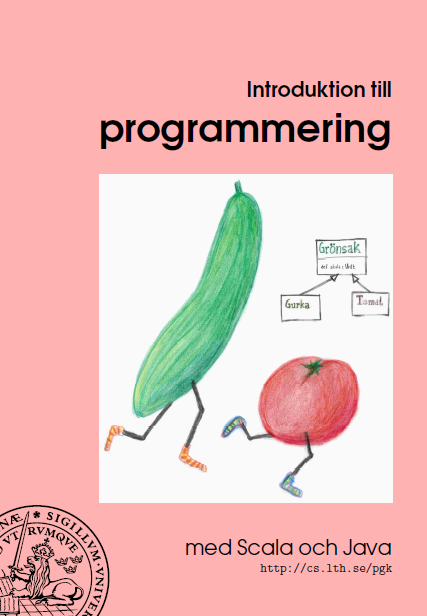
\includegraphics[width=0.65\textwidth]{../img/compendium-front-page.png}
\begin{itemize}
\item \Emph{Kompendium} med övningar \& laborationer, trycks \& säljs av inst. på beställning
\item Föreläsningsbilder
\item Nätresurser enl. länkar

\end{itemize}
\end{minipage}
\hskip1em\begin{minipage}{0.5\textwidth}\SlideFontSize{8}{10}
Bra, men ej nödvändig, \Emph{bredvidläsning}:\\ 
-- för \Emph{nybörjare}:
\vskip0.2mm

\includegraphics[width=0.33\textwidth]{../img/lewisbook.jpg}\hskip4mm
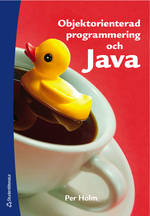
\includegraphics[width=0.33\textwidth]{../img/ankbok.jpg}

\noindent -- för de som \Emph{redan kodat} en del:
\vskip0.7mm
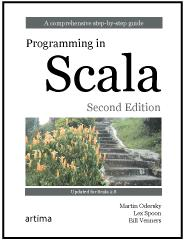
\includegraphics[width=0.45\textwidth]{../img/pinsbook.jpg}\hskip4mm
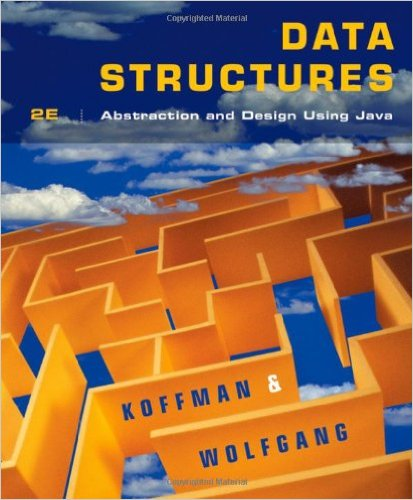
\includegraphics[width=0.47\textwidth]{../img/koffmanbook.jpg}
\end{minipage}
\end{Slide}

\ifkompendium
\noindent Kompendiet är den huvudsakliga kurslitteraturen och definierar kursinnehållet. Föreläsningar, övningar och laborationer i kompendiet är kursens primära kunskapskällor, tillsammans med de öppna resurser på nätet som kompendiet hänvisar till. Kompendiet är öppen källkod och du välkomnas varmt att bidra!

Om du gärna vill ha en eller flera mer traditionella läroböcker som bredvidläsning rekommenderas följande:
\begin{itemize}[noitemsep, leftmargin=*]
\item För de som aldrig kodat, och vill läsa om kodning från grunden:
\begin{itemize}[nolistsep]
\item ''Introduction to Programming and Problem-Solving Using Scala, Second Edition'', Mark C. Lewis, Lisa Lacher.  {\href{https://www.crcpress.com/Introduction-to-Programming-and-Problem-Solving-Using-Scala-Second-Edition/Lewis-Lacher/p/book/9781498730952}{www.crcpress.com/Introduction-to-Programming-and-Problem-Solving-Using-Scala-Second-Edition/Lewis-Lacher/p/book/9781498730952}}
\item ''Objektorienterad programmering och Java'', Per Holm, Tredje upplagan (2007). \href{https://www.studentlitteratur.se/#6735}{www.studentlitteratur.se/\#6735}
\end{itemize}
\item För de som redan kodat en hel del i ett objektorienterat språk:
\begin{itemize}[nolistsep, noitemsep]
\item ''Programming in Scala, Third Edition -- A comprehensive step-by-step guide'', Martin Odersky, Lex Spoon, and Bill Venners. \\ \href{http://www.artima.com/shop/programming_in_scala_3ed}{www.artima.com/shop/programming\_in\_scala\_3ed} 
\item ''Data Structures: Abstraction and Design Using Java, 3rd Edition'', Elliot B. Koffman, Paul A. T. Wolfgang. \\
\href{http://eu.wiley.com/WileyCDA/WileyTitle/productCd-1119186528.html}{http://eu.wiley.com/WileyCDA/WileyTitle/productCd-1119186528.html}
\end{itemize}
\end{itemize}
Dessa läroböcker följer inte direkt kursens upplägg vad gäller omfång och progression och du får själv göra den nyttiga hemläxan att koppla  deras innehåll till det vi går igenom i kursens olika moduler.

\else
\begin{Slide}{Beställning av kompendium och snabbreferens}\SlideFontSmall
\begin{itemize}
\item \Emph{Kompendiet} finns i pdf för fri nedladdning enl. CC-BY-SA, men det \Alert{rekommenderas starkt} att du köper den tryckta bokversionen.
\item Det är mycket lättare att ha övningar och labbar \Alert{på papper} \Emph{bredvid skärmen}, när du ska tänka, koda och plugga!
\item \Emph{Snabbreferensen} finns också i pdf men du behöver ha en tryckt version eftersom det är \Alert{enda tillåtna hjälpmedlet} på skriftliga kontrollskrivningen och tentamen.
\item Kompendiet och snabbreferens trycks här i E-huset och säljs av institutionen till självkostnadspris. Pris för kompendium+snabbreferens \Alert{beror på hur många som beställer}.
\item Snabbreferens enbart kostar 10 kr.
\item Skriv upp dig på listan -- tryckning sker efter beställning.
\item Du betalar \Alert{kontant} med \Emph{jämna pengar} på cs expedition, våning 2.
\end{itemize}
\end{Slide}
\fi

\ifkompendium\else
\begin{Slide}{Personal}\SlideFontSmall
\begin{description}
\item [\bfseries Kursansvarig:] ~\\Björn Regnell, bjorn.regnell@cs.lth.se
\item [\bfseries Kurssekreterare:]  ~\\Lena Ohlsson \\Exp.tid 09.30 -- 11.30 samt 12.45 -- 13.30
\item [\bfseries Handledare:] ~\\
\Emph{Doktorander}: \\ 
Tekn. Lic. Maj Stenmark, Gustav Cedersjö\\
\Emph{Teknologer}: \\
Anders Buhl, 
Anna Palmqvist Sjövall, 
Anton Andersson,
Cecilia Lindskog, 
Emil Wihlander, 
Erik Bjäreholt, 
Erik Grampp, 
Filip Stjernström, 
Fredrik Danebjer, 
Henrik Olsson, 
Jakob Hök, 
Jonas Danebjer, 
Måns Magnusson, 
Oscar Sigurdsson, 
Oskar Berg, 
Oskar Widmark, 
Sebastian Hegardt, 
Stefan Jonsson, 
Tom Postema, 
Valthor Halldorsson
\end{description}
\end{Slide}
\fi

\begin{Slide}{Föreläsningsanteckningar}
\begin{itemize}
\item Föreläsningsanteckningar utvecklas under kursens gång
\item Några av bilderna finns i kompendiet
\item Alla bilder läggs ut här: \\
\href{https://github.com/lunduniversity/introprog/tree/master/slides}{github.com/lunduniversity/introprog/tree/master/slides} \\
och uppdateras kontinuerligt allt eftersom de utvecklas
\item Förslag på förbättringar välkomna!
\end{itemize}
\end{Slide}

\begin{Slide}{Kursmoment --- varför?}\SlideOnly{\footnotesize}
\begin{itemize}
\item \Emph{Föreläsningar}: skapa översikt, ge struktur, förklara teori, svara på frågor, motivera varför
\item \Emph{Övningar}: \Alert{förbereda} laborationerna, bearbeta teorins olika delar med avgränsade deluppgifter, \Emph{grundövningar} för alla, \Emph{extraövningar} om du vill/behöver öva mer, \Emph{fördjupningsövningar} om du vill gå djupare 
\item \Emph{Laborationer}: \Alert{obligatoriska}, sätta samman teorins delar i ett större program; lösningar redovisas för handledare; gk på alla för att få tenta, 
\item \Emph{Resurstider}: få hjälp med övningar och laborationsförberedelser av handledare, fråga vad du vill
\item \Emph{Samarbetsgrupper}: grupplärande genom samarbete, hjälpa varandra 
\item \Emph{Kontrollskrivning}: \Alert{obligatorisk}, diagnostisk, kamraträttad; kan ge samarbetsbonuspoäng till tentan
\item \Emph{Individuell projektuppgift}: \Alert{obligatorisk}, du visar att du kan skapa ett större program självständigt; redovisas för handledare
\item \Emph{Tentamen}: \Alert{obligatorisk}, skriftlig, enda hjälpmedel: snabbreferensen\\   \url{http://cs.lth.se/pgk/quickref}
\end{itemize}
\end{Slide}

\ifkompendium\else
\begin{Slide}{Detta är bara början... }
Exempel på efterföljande kurser som bygger vidare på denna:
\begin{itemize}
\item Årskurs 1
\begin{itemize}
\item Programmeringsteknik -- fördjupningskurs
\item Utvärdering av programvarusystem
\item Diskreta strukturer
\end{itemize}
\item Årskurs 2
\begin{itemize}
\item Objektorienterad modellering och design
\item Programvaruutveckling i grupp
\item Algoritmer, datastrukturer och komplexitet
\item Funktionsprogrammering
\end{itemize}
\end{itemize}
\end{Slide}


\begin{Slide}{Registrering}
\begin{itemize}
\item Fyll i listan som skickas runt.
\item Kryssa i kolumnen \Emph{Ska gå} om du ska gå kursen\footnote{\scriptsize D1:a som redan gått motsvarande högskolekurs? Uppsök studievägledningen}\footnote{\scriptsize D2:a eller äldre som vill bli omregistrerad? Prata med kursansvarig på rasten}
\item Kryssa i kolumnen \Emph{Kursombud} om du kan tänka dig att vara kursombud under kursens gång
\begin{itemize}
\item Alla LTH-kurser ska utvärderas under kursens gång och efter kursens slut.
\item Till det behövs kursombud -- ungefär 2 D-are och 2 W-are.
\item Ni kommer att bli kontaktade av studierådet. \\SRD ordf: Amelia Andersson
\end{itemize}
\end{itemize}
\end{Slide}

%%%
\begin{Slide}{Förkunskaper}
\begin{itemize}
\item Förkunskaper $\neq$ Förmåga
\item Varken kompetens eller personliga egenskaper är statiska 
\item ''Programmeringskompetens'' är inte \textit{en} enda enkel förmåga utan en komplex sammansättning av flera olika förmågor som utvecklas genom hela livet
\item Ett innovativt utvecklar\Alert{team} behöver många olika kompetenser för att vara framgångsrikt
\end{itemize}
\end{Slide}

%%%
\begin{Slide}{Förkunskapsenkät}
\begin{itemize}
\item Om du inte redan gjort det fyll i förkunskapsenkäten \Alert{snarast}:
\url{http://cs.lth.se/pgk/survey} 
\item Dina svar behandlas internt och all redovisad statistik anonymiseras.
\item Enkäten ligger till grund för randomiserad gruppindelning i samarbetsgrupper, så att det blir en spridning av förkunskaper inom gruppen.
\item Gruppindelnig publiceras här: \\ \url{http://cs.lth.se/pgk/grupper/}
\end{itemize}
\end{Slide}

\begin{Slide}{Samarbetgrupper}\footnotesize
\begin{itemize}
\item Ni delas in i \Emph{samarbetsgrupper} om ca 5 personer baserat på förkunskapsenkäten, så att olika förkunskapsnivåer sammanförs
\item Några av laborationerna är mer omfattande \Emph{grupplabbar} och kommer att göras i samarbetsgrupperna \\ \vspace{1em}
\item Kontrollskrivningen i halvtid kan ge \Emph{samarbetsbonus} (max 5p) som adderas till ordinarie tentans poäng (max 100p) med medelvärdet av gruppmedlemmarnas individuella kontrollskrivningspoäng 
\scriptsize \parbox{7cm}{Bonus $b$ för varje person i en grupp med $n$ medlemmar med $p_i$ poäng vardera på kontrollskrivningen:} 
 \hspace{5mm} $\displaystyle b = \sum\limits_{i=1}^n \frac{p_i}{n}$
\end{itemize}
\end{Slide}

\fi

%%%
\begin{Slide}{Varför studera i samarbetsgrupper?}

Huvudsyfte: \Emph{Bra lärande!}

\begin{itemize}
\item Pedagogisk forskning stödjer tesen att lärandet blir mer djupinriktat om det sker i utbyte med andra
\item Ett studiesammanhang med höga ambitioner och respektfull gemenskap gör att vi \Emph{når mycket längre}
\item Varför ska du som redan kan mycket aktivt dela med dig av dina kunskaper?
\begin{itemize}
\item Förstå bättre själv genom att förklara för andra
\item Träna din pedagogiska förmåga
\item Förbered dig för ditt kommande yrkesliv som mjukvaruutvecklare 
\end{itemize}
\end{itemize}
\end{Slide}

%%%

\ifkompendium\else
\begin{Slide}{Samarbetskontrakt}
Gör ett skriftligt \href{https://github.com/bjornregnell/lth-eda016-2015/blob/master/assignments/collaboration-contract.tex}{\bf samarbetskontrakt} med dessa och ev. andra punkter som ni också tycker bör ingå:
\begin{enumerate}
\item Återkommande mötestider per vecka
\item Kom i tid till gruppmöten
\item Var väl förberedd genom självstudier inför gruppmöten
\item Hjälp varandra att förstå, men ta inte över och lös allt
\item Ha ett respektfullt bemötande även om ni har olika åsikter
\item Inkludera alla i gemenskapen
\end{enumerate}

Diskutera hur ni ska uppfylla dessa innan alla skriver på. \\ Ta med samarbetskontraktet och visa för handledare på labb 1.

\vskip1em

\Alert{Om arbetet i samarbetsgruppen inte fungerar ska ni mejla kursansvarig och boka mötestid!}
\end{Slide}

\begin{Slide}{Bestraffa inte frågor!}
\begin{itemize}
\item Det finns bättre och sämre frågor vad gäller hur mycket man kan lära sig av svaret, men \Emph{all undran är en chans} att i dialog utbyta erfarenheter och lärande
\item Den som frågar \Emph{vill veta} och berättar genom frågan något om nuvarande kunskapsläge
\item Den som svarar får chansen att \Emph{reflektera} över vad som kan vara svårt och olika vägar till djupare förståelse
\item I en hälsosam lärandemiljö är det \Emph{helt tryggt} att visa att man ännu inte förstår, att man gjort ''fel'', att man har mer att lära, etc. 
\item Det är viktigt att våga försöka även om det blir ''fel'':\\ \Emph{det är ju då man lär sig!}
\end{itemize}
\end{Slide}

%%%
\begin{Slide}{Plagiatregler}
Läs dessa regler noga och diskutera i samarbetsgrupperna:
\begin{itemize}
\footnotesize
\item \url{http://cs.lth.se/utbildning/samarbete-eller-fusk/}
\item \url{http://cs.lth.se/utbildning/foereskrifter-angaaende-obligatoriska-moment/}
\end{itemize}
Ni ska lära er genom \Emph{eget arbete} och genom  \Emph{bra samarbete}. Samarbete gör att man lär sig bättre, men man lär sig inte av att bara kopiera andras lösningar. Plagiering är förbjuden och kan medföra disciplinärende och avstängning.
\end{Slide}

\fi %%%%%%%%%%%%%%%%%%%%%%%%%%%%%%%%

%%%
\begin{Slide}{En typisk kursvecka}
\begin{enumerate}
\item Gå på \Emph{föreläsningar} på \Alert{måndag--tisdag}
\item Jobba med \Emph{individuellt} med teori, övningar, labbförberedelser på  \Alert{måndag--torsdag}
\item Kom till \Emph{resurstiderna} och få hjälp och tips av handledare och kurskamrater på \Alert{onsdag--torsdag}
\item Genomför den obligatoriska \Emph{laborationen} på \Alert{fredag}
\item Träffas i \Emph{samarbetsgruppen} och hjälp varandra att förstå mer och fördjupa lärandet, förslagsvis på återkommande tider varje vecka då alla i gruppen kan
\end{enumerate}
Se detaljerna och undantagen i schemat: \href{http://cs.lth.se/pgk/schema}{cs.lth.se/pgk/schema}
\end{Slide}

\ifkompendium\else  %%%%%%%%%%%%%%%%%%%%%%%%%
%%%
\begin{Slide}{Laborationer}\footnotesize
\begin{itemize}
\item \Alert{Programmering lär man sig bäst genom att programmera...}
\item Labbarna är \Emph{individuella} (utom 2) och \Emph{obligatoriska}
\item Gör övningarna och labbförberedelserna noga \textit{innan} själva labben -- detta är ofta helt nödvändigt för att du ska hinna klart. Dina labbförberedelserna kontrolleras av handledare under labben.
\item Är du sjuk? Anmäl det \Alert{före} labben till \url{bjorn.regnell@cs.lth.se}, \\ få hjälp på resurstid och redovisa på resurstid (eller labbtid, när handledaren har tid över)
\item Hinner du inte med hela? Se till att handledaren noterar din närvaro, och fortsätt på resurstid och ev. uppsamlingstider.
\item Läs noga anvisningarna i kompendiet
\item Laborationstiderna är gruppindelade enligt \href{http://cs.lth.se/eda016/schema/}{schemat}. Du ska gå till den tid och den sal som motsvarar din \href{http://cs.lth.se/eda016/grupper/}{grupp}.
\end{itemize}
\end{Slide}

%%%
\begin{Slide}{Resurstider}
\begin{itemize}
\item På resurstiderna får du hjälp med övningar och laborationsförberedelser
\item Kom till minst en resurstid per vecka (se \href{http://cs.lth.se/eda016/schema/}{schema})
\item Handledare gör ibland \Emph{genomgångar} för alla under resurstiderna. Tipsa om handledare om vad du finner svårt.
\item Resurstiderna är inte gruppindelade i schemat. Du får i mån av plats gå på flera resurstider per vecka. Om det blir fullt i ett rum prioriteras dessa grupper för att minimera schemakrockar: 
\end{itemize}
\begin{table}[]
\centering\scriptsize
\begin{tabular}{lllll}
Tid Lp1 & Sal & Grupper med prio \\
\hline
Ons 10-12 v1-7 & Hacke  &   09 \& 10 \\
Ons 13-15 v1-7 & Hacke  &   07 \& 08  \\
Ons 15-17 v1-7 & Panter  & 05 \& 06   \\
Ons 15-17 v1-7 & Val       &  03 \& 04   \\
Tor 13-15 v1-7 & Mars     & 01 \& 02  \\
Tor 15-17 v1-7 & Mars     & 11 \& 12 \\ 
\end{tabular}
\end{table}
\end{Slide}

\fi
%!TEX root = ../lect-week01.tex

%%%%%%%%%%%%%%%%%%%%%%%%%%%%%%%%%%%%%%
\Subsection{Om programmering}

%%%

\begin{Slide}{Att skapa koden som styr världen}
\begin{multicols}{2}\footnotesize
I stort sett alla delar av samhället är beroende av programkod:
\begin{itemize}\scriptsize
\item kommunikation
\item transport
\item byggsektorn
\item statsförvaltning
\item finanssektorn
\item media \& underhållning
\item sjukvård
\item övervakning
\item integritet
\item upphovsrätt
\item miljö \& energi
\item sociala relationer
\item utbildning 
\item ...
\end{itemize}
\columnbreak %---------
Hur blir ditt framtida yrkesliv som systemutvecklare?
\begin{itemize}
\item  Redan nu är det en skriande brist på utvecklare och bristen blir bara värre och värre... \\
  \href{http://computersweden.idg.se/2.2683/1.634770/rekrytera-utvecklare}{CS 2015-08-17}
\item Störst brist är det på kvinnliga utvecklare: \\
\href{http://www.dn.se/ekonomi/it-branschen-hotas-av-brist-pa-kvinnor/}{DN 2015-04-02}
\item Global kompetensmarknad \\ 
  \href{http://computersweden.idg.se/2.2683/1.630901/det-finns-programmerare-och-sa-finns-det-programmerare}{CS 2015-06-14}\\
   \href{http://computersweden.idg.se/2.2683/1.634700/7-satt-att-bli-en-battre-programmerare}{CS 2015-08-15}
\end{itemize}
\end{multicols}
\end{Slide}


\ifkompendium\noindent
{\scriptsize
\url{http://computersweden.idg.se/2.2683/1.634770/rekrytera-utvecklare}\\
\url{http://www.dn.se/ekonomi/it-branschen-hotas-av-brist-pa-kvinnor}\\
\url{http://computersweden.idg.se/2.2683/1.630901/det-finns-programmerare-och-sa-finns-det-programmerare}
\url{http://computersweden.idg.se/2.2683/1.634700/7-satt-att-bli-en-battre-programmerare}
}
\fi

\begin{Slide}{Utveckling av mjukvara i praktiken}
\begin{itemize}
\item \Emph{Inte bara kodning:} kravbeslut, releaseplanering, design, test, versionshantering, kontinuerlig integration, driftsättning, återkoppling från dagens användare, ekonomi \& investering, gissa om morgondagens användare, ... 
\item \Emph{Teamwork:} Inte ensamma hjältar utan autonoma team i decentraliserade organisationer med innovationsuppdrag
\item \Emph{Snabbhet:} Att koda innebär att hela tiden uppfinna nya ''byggstenar'' som ökar organisationens förmåga att snabbt skapa värde med hjälp av mjukvara. Öppen källkod. Skapa kraftfulla API:er.
\item \Emph{Livslångt lärande:} Lär nytt och dela med dig hela tiden. Exempel på pedagogisk utmaning: hjälp andra förstå och använda ditt API $\implies$ \textit{Samarbetskultur}
\end{itemize}
\end{Slide}

\ifkompendium\else
\SlideImg{Programming unplugged: Två frivilliga?}{../img/unplugged}
\SlideImg{Editera och exekvera ett program}{../img/kojo}
\fi


%%%%%%%%%%%%%%%%%%%%%%%%%%%%%%%%%%%%%%
\ifkompendium\else
\Subsection{Meddelande från \href{http://lth.se/code}{Code@LTH}} 
\fi

\Lecture{2}{Kodstruktur}
%!TEX encoding = UTF-8 Unicode
%!TEX root = ../lect-week02.tex

%\Subsection{Samlingar och loopar}
\Subsection{Datastrukturer och kontrollstrukturer}


\begin{Slide}{Vad är en datastruktur?}\SlideFontSmall
\begin{itemize}
\item En \href{https://sv.wikipedia.org/wiki/Datastruktur}{datastruktur} är en struktur för organisering av data som...
\begin{itemize}\SlideFontTiny
\item kan innehålla \Alert{många} element,
\item kan refereras till med \Alert{ett} enda namn, och
\item ger möjlighet att komma åt de enskilda elementen.
\end{itemize}

\item En \Emph{samling} \Eng{collection} är en datastruktur som kan innehålla många element av \Alert{samma typ}.

\item Exempel på olika samlingar där elementen är organiserade på olika vis: \\ 
\vspace{0.5em}
\begin{tabular}{l c}
\Emph{Lista} & 
\includegraphics[width=5cm]{../img/list.pdf} \\
\Emph{Träd}  & 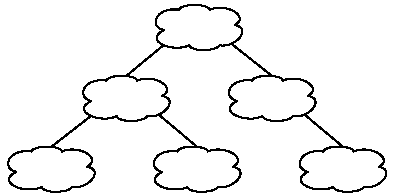
\includegraphics[width=2.2cm]{../img/tree.pdf} \\
\Emph{Graf}  & 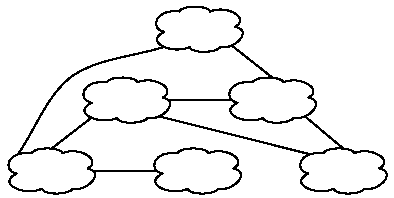
\includegraphics[width=2.2cm]{../img/graph.pdf} \\
\end{tabular}
\end{itemize}
{
\SlideFontTiny \vspace{1em }\hskip2em
Mer om listor \& träd \href{http://cs.lth.se/edaa01vt}{fördjupningskursen}. 
Mer om träd, grafer i \href{http://cs.lth.se/edaa40}{Diskreta strukturer.}
}

\end{Slide} 


\begin{Slide}{Vad är en vektor?}\SlideFontSmall
En \Emph{vektor}\footnote{Vektor kallas ibland på svenska även \href{https://sv.wikipedia.org/wiki/F\%C3\%A4lt_\%28datastruktur\%29}{fält}, men det skapar stor förvirring eftersom det engelska ordet \emph{field} ofta används för \emph{attribut} (förklaras senare).} 
\Eng{vector, \href{https://en.wikipedia.org/wiki/Array_data_structure}{array}} är en \Emph{samling} som är \Alert{snabb} att \Emph{indexera} i. 
Åtkomst av element sker med \code{apply(platsnummer)}: 

\begin{REPL}
scala> val heltal = Vector(42, 13, -1, 0 , 1)
heltal: scala.collection.immutable.Vector[Int] = Vector(42, 13, -1, 0, 1)

scala> heltal.apply(0)
res0: Int = 42

scala> heltal(1)    // man kan skippa .apply
res1: Int = 13

scala> heltal(5)
java.lang.IndexOutOfBoundsException: 5
  at scala.collection.immutable.Vector.checkRangeConvert(Vector.scala:132)
\end{REPL}
Utelämnar du \code{.apply} så gör kompilatorn anrop av \code{apply} ändå om det går.
\end{Slide}

\begin{Slide}{En konceptuell bild av en vektor}

\begin{REPLnonum}
scala> val heltal = Vector(42, 13, -1, 0 , 1)

scala> heltal(0)
res0: Int = 42
\end{REPLnonum}

\begin{tikzpicture}[font=\ttfamily]
\matrix [matrix of nodes, row sep=0, column 2/.style={nodes={rectangle,draw,minimum width=3em}}] (var) at (0cm, 2.8cm)
{
heltal   &  \makebox(16,12){ }\\
};
\matrix [matrix of nodes, draw=black,row sep=0, column 2/.style={nodes={rectangle,draw,minimum width=4em}}] (vec) at (4cm, 1cm)
{
\textit{plats} &  \\
0   &  \makebox(16,12){42}\\
1   &  \makebox(16,12){13}\\
2   &  \makebox(16,12){-1}\\
3   &  \makebox(16,12){0}\\
4   &  \makebox(16,12){1}\\
};
\filldraw[black] (0.7cm,2.8cm) circle (3pt) node[] (ref) {};
 \draw [arrow] (ref) -- (vec);
\end{tikzpicture}

%\vspace{1em} Elementen ligger på rad någonstans i minnet.
\end{Slide}



\begin{Slide}{En samling strängar}

\begin{itemize}
\item En vektor kan lagra många värden av samma typ. 
\item Elementen kan vara till exempel heltal eller strängar. 
\item Eller faktiskt vad som helst. 
\end{itemize}

\begin{REPL}
scala> val grönsaker = Vector("gurka","tomat","paprika","selleri")
grönsaker: scala.collection.immutable.Vector[String] = Vector(gurka, tomat, paprika, selleri)

scala> val g = grönsaker(1)
g: String = tomat

scala> val xs = Vector(42, "gurka", true, 42.0)
xs: scala.collection.immutable.Vector[Any] = Vector(42, gurka, true, 42.0)


\end{REPL}

\end{Slide}

\begin{Slide}{Vad är en kontrollstruktur?}
\begin{itemize}
\item En \Emph{kontrollstruktur} påverkar \Alert{sekvensen}.
\begin{itemize}
\item[] Exempel på inbyggda kontrollstrukturer: 
\\\vspace{0.5em}\code{for}-sats, \code{while}-sats
\end{itemize}

\item[]

\item I Scala kan man definiera \Emph{egna} kontrollstrukturer.
\begin{itemize}
\item[] Exempel: \code{upprepa} som du använt i Kojo
\\\vspace{0.5em}\code|upprepa(4){fram; höger}|
\end{itemize}
\end{itemize}
\end{Slide}


\begin{Slide}{Mitt första program: en oändlig loop på ABC80}
\begin{columns}
\begin{column}{0.8\textwidth}
\begin{verbatim}
10 print "hej"
20 goto 10
\end{verbatim}
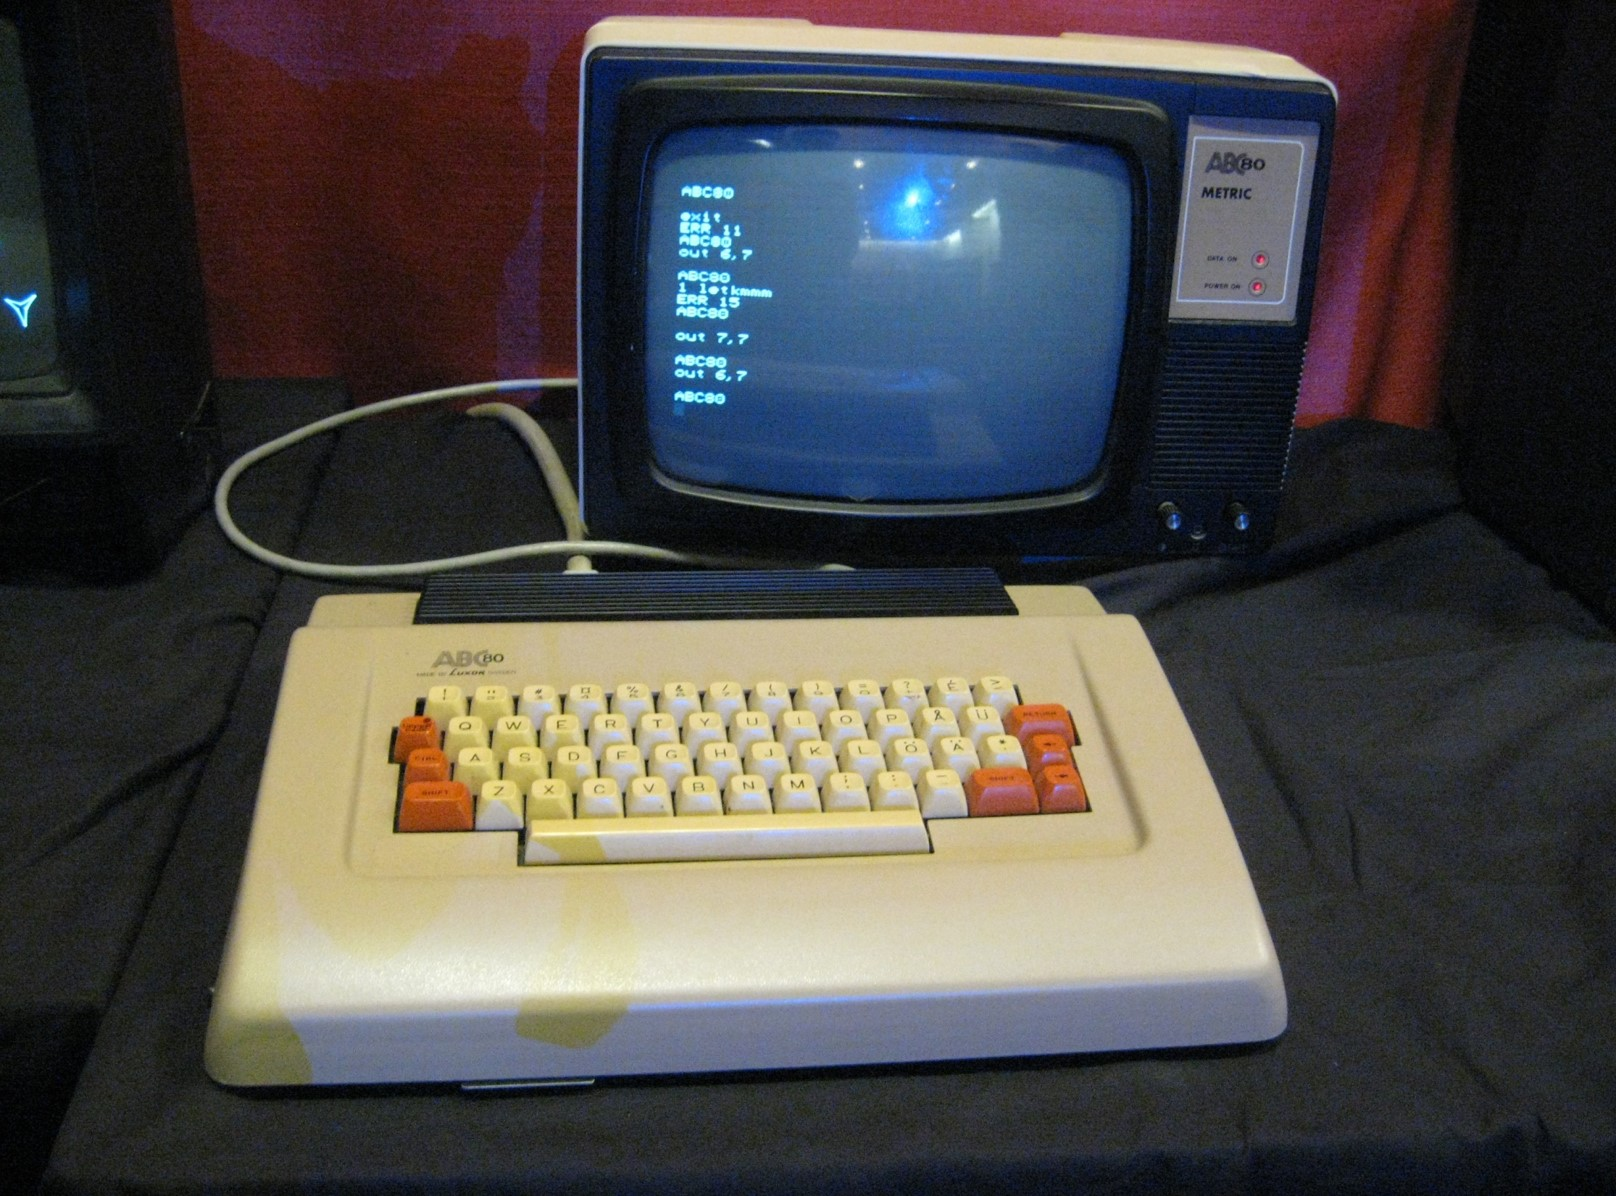
\includegraphics[width=0.8\textwidth]{../img/abc80.jpg}
\end{column}
\begin{column}{0.3\textwidth}
\pause
\begin{verbatim}
hej
hej
hej
hej
hej
hej
hej
hej
hej
hej
hej
hej
<Ctrl+C>
\end{verbatim}

\end{column}
\end{columns}
\end{Slide}


\begin{Slide}{Loopa genom elementen i en vektor}
En \code{for}-\Emph{sats} som skriver ut alla element i en vektor:
\begin{REPL}
scala> val grönsaker = Vector("gurka","tomat","paprika","selleri")

scala> for (g <- grönsaker) println(g)
gurka
tomat
paprika
selleri

\end{REPL}

\end{Slide}


\begin{Slide}{Bygga en ny samling från en befintlig med for-uttryck}
Ett \code{for}-\code{yield}-\Emph{uttryck} som \Emph{skapar en \Alert{ny} samling}.

\begin{Code}[basicstyle=\ttfamily\fontsize{12}{14}\selectfont]
for (g <- grönsaker) yield "god " + g
\end{Code}

\begin{REPL}
scala> val grönsaker = Vector("gurka","tomat","paprika","selleri")

scala> for (g <- grönsaker) yield "god " + g
res0: scala.collection.immutable.Vector[String] = 
  Vector(god gurka, god tomat, god paprika, god selleri)

scala> val åsikter = for (g <- grönsaker) yield s"god $g"
åsikter: scala.collection.immutable.Vector[String] = 
  Vector(god gurka, god tomat, god paprika, god selleri)
\end{REPL}

\end{Slide}


\begin{Slide}{Samlingen \code{Range} håller reda på intervall}
\begin{itemize}
\item Med en \code{Range(start, slut)} kan du skapa ett intervall: \\ från och med \code{start} till (men inte med) \code{slut}
\end{itemize}

\begin{REPLnonum}
scala> Range(0, 42)
res0: scala.collection.immutable.Range = 
  Range(0, 1, 2, 3, 4, 5, 6, 7, 8, 9, 10, 11, 12, 13, 14, 
    15, 16, 17, 18, 19, 20, 21, 22, 23, 24, 25, 26, 27, 28, 
    29, 30, 31, 32, 33, 34, 35, 36, 37, 38, 39, 40, 41)
\end{REPLnonum}

\begin{itemize}
\item Men alla värden däremellan skapas inte förrän de behövs:
\end{itemize}

\begin{REPL}
scala> val jättestortIntervall = Range(0, Int.MaxValue)
jättestortIntervall: scala.collection.immutable.Range = Range(0, 1, 2, 3, 4, 5, ...

scala> jättestortIntervall.end
res1: Int = 2147483647

scala> jättestortIntervall.toVector
java.lang.OutOfMemoryError: GC overhead limit exceeded
\end{REPL}

\end{Slide}

\begin{Slide}{Loopa med Range}
\code{Range} används i for-lopar för att hålla reda på antalet rundor.
\begin{REPLnonum}
scala> for (i <- Range(0, 6)) print(" gurka " + i)
 gurka 0 gurka 1 gurka 2 gurka 3 gurka 4 gurka 5 
\end{REPLnonum}
Du kan skapa en \code{Range} med \code{until} efter ett heltal:
\begin{REPLnonum}
scala> 1 until 7
res1: scala.collection.immutable.Range = 
  Range(1, 2, 3, 4, 5, 6)

scala> for (i <- 1 until 7) print(" tomat " + i) 
 tomat 1 tomat 2 tomat 3 tomat 4 tomat 5 tomat 6

\end{REPLnonum}
\end{Slide}

\begin{Slide}{Loopa med Range skapad med \texttt{to}}

Med \code{to} efter ett heltal får du en \code{Range} till och \Emph{med} sista:
\begin{REPLnonum}
scala> 1 to 6
res2: scala.collection.immutable.Range.Inclusive = 
  Range(1, 2, 3, 4, 5, 6)

scala> for (i <- 1 to 6) print(" gurka " + i) 
 gurka 1 gurka 2 gurka 3 gurka 4 gurka 5 gurka 6
 
\end{REPLnonum}


\end{Slide}



\begin{Slide}{Vad är en \code{Array} i JVM?}


\begin{itemize}
\item En \code{Array} liknar en \code{Vector} men har en särställning i JVM:
\begin{itemize}
\item Lagras som en sekvens i minnet på efterföljande adresser.
\item \Emph{Fördel}: snabbaste samlingen för element-access i JVM.
\item Men det finns en hel del \Alert{nackdelar} som vi ska se senare.
\end{itemize}

\end{itemize}

\begin{REPLnonum}
scala> val heltal = Array(42, 13, -1, 0 , 1)
\end{REPLnonum}

\begin{tikzpicture}[font=\ttfamily,scale=0.75, every node/.style={scale=0.75}]
\matrix [matrix of nodes, row sep=0, column 2/.style={nodes={rectangle,draw,minimum width=3em}}] (var) at (0cm, 2.8cm)
{
heltal   &  \makebox(16,12){ }\\
};
\matrix [matrix of nodes, draw=black,row sep=0, column 2/.style={nodes={rectangle,draw,minimum width=4em}}] (vec) at (4cm, 1cm)
{
\textit{plats} &  \\
0   &  \makebox(16,12){42}\\
1   &  \makebox(16,12){13}\\
2   &  \makebox(16,12){-1}\\
3   &  \makebox(16,12){0}\\
4   &  \makebox(16,12){1}\\
};
\filldraw[black] (0.7cm,2.8cm) circle (3pt) node[] (ref) {};
 \draw [arrow] (ref) -- (vec);
\end{tikzpicture}
\end{Slide}

\begin{Slide}{Några likheter \& skillnader mellan \texttt{Vector} och \texttt{Array}}\SlideFontSmall
\begin{multicols}{2}
\begin{REPL}[numbers=none]
scala> val xs = Vector(1,2,3)
\end{REPL}

\columnbreak

\begin{REPL}[numbers=none]
scala> val xs = Array(1,2,3)
\end{REPL}
\end{multicols}


Några likheter mellan \texttt{Vector} och \texttt{Array}
\begin{itemize}
\item Båda är samlingar som kan innehålla många element.

\item Med båda kan man snabbt accessa vilket element som helst: \code{xs(2)}

\item Båda har en fix storlek efter allokering.
\end{itemize}

Några viktiga skillnader:
\begin{multicols}{2}
\Emph{Vector}
\begin{itemize}
\item Är \Emph{oföränderlig}: du kan lita på att elementreferenserna aldrig någonsin kommer att ändras.

\item Är \Emph{snabb på att skapa en delvis förändrad kopia}, t.ex. tillägg/borttagning/uppdatering mitt i sekvensen.

\end{itemize}


\columnbreak

\Alert{Array}
\begin{itemize}
\item Är \Alert{föränderlig}: \code{xs(2) = 42}

\item Är \Alert{snabb} om man bara vill läsa eller skriva på befintliga platser.

\item Är \Alert{långsam} om man vill lägga till eller ta bort element mitt i sekvensen.

\end{itemize}
\end{multicols}
\end{Slide}



\Subsection{Huvudprogram med \texttt{main} i Scala och Java}

\begin{Slide}{Ett minimalt fristående program i Scala och Java}
Nedan Scala-kod skrivs i en editor, spara med valfritt filnamn:
\begin{Code}
// this is Scala 

object Hello {
  def main(args: Array[String]): Unit = {
    println("Hejsan scala-appen!")
  }
}
\end{Code}

\pause
\vspace{1em}
Nedan Java-kod skrivs i en editor, filen \Alert{måste} heta \texttt{Hi.java}

\begin{Code}[language=Java]
// this is Java 

public class Hi {
    public static void main(String[] args) {
        System.out.println("Hejsan Java-appen!");
    }
}
\end{Code}

\end{Slide}


\begin{Slide}{Loopa genom en samling med en \texttt{while}-sats}
\begin{REPLnonum}
scala> val xs = Vector("Hej","på","dej","!!!")
xs: scala.collection.immutable.Vector[String] = 
  Vector(Hej, på, dej, !!!)

scala> xs.size
res0: Int = 4

scala> var i = 0
i: Int = 0

scala> while (i < xs.size) { println(xs(i)); i = i + 1 }
Hej
på
dej
!!!
\end{REPLnonum}
\end{Slide}


\begin{Slide}{Loopa genom argumenten i ett Scala-huvudprogram}
Skriv denna kod och spara i filen \texttt{helloargs.scala}
\begin{REPL}[numbers=none]
$ gedit helloargs.scala
\end{REPL}
\begin{Code}
object HelloScalaArgs {
  def main(args: Array[String]): Unit = {
    var i = 0
    while (i < args.size) { 
      println(args(i))
      i = i + 1
    }
  }
}
\end{Code}
Kompilera och kör:
\begin{REPL}
$ scalac helloargs.scala
$ scala HelloScalaArgs hej gurka tomat 
hej
gurka
tomat
\end{REPL}
\end{Slide}


\begin{Slide}{Loopa genom argumenten i ett Java-huvudprogram}
\begin{REPL}[numbers=none]
$ gedit HelloJavaArgs.java
\end{REPL}
\begin{Code}[language=Java]
// this is Java 

public class HelloJavaArgs {
    public static void main(String[] args) {
    int i = 0;
    while (i < args.length) { 
      System.out.println(args[i]);
      i = i + 1;
    }
  }
}
\end{Code}
Kompilera och kör:
\begin{REPL}
$ javac HelloJavaArgs.scala
$ java HelloJavaArgs hej gurka tomat 
hej
gurka
tomat
\end{REPL}

\end{Slide}


\begin{Slide}{Scala-skript}
\begin{itemize}
\item Skala-kod kan köras som ett \Emph{skript}.\footnote{\SlideFontTiny Du får prova detta på övningen. Vi kommer mest att köra kompilerat i kursen, då Scala-skript saknar mekanism för inkludering av andra skript. Men det finns ett öppenkällkodsprojekt som löser det: \url{http://www.lihaoyi.com/Ammonite/}
}
\item Ett skript kompileras varje gång innan det körs och maskinkoden sparas inte som vid vanlig kompilering.
\item Då behövs ingen \code{main} och inget \code{object}
\end{itemize}

\begin{Code}[basicstyle=\ttfamily\fontsize{10}{12}\selectfont]
// spara nedan i filen 'myscript.scala'

println("Hejsan argumnet!")
for (arg <- args) println(arg)
\end{Code}

\begin{REPLnonum}
$ scala myscript.scala
\end{REPLnonum}


\end{Slide}



\Subsection{Algoritmer: stegvisa lösningar}

\begin{Slide}{Vad är en algoritm?}
En \href{https://sv.wikipedia.org/wiki/Algoritm}{algoritm} är en sekvens av instruktioner som beskriver \\hur man löser ett problem.\\
\vspace{1em}
\Emph{Exempel}: 
\begin{itemize}
\item	 baka en kaka 
\pause\item räkna ut din pensionsprognos 
\pause\item köra bil 
\pause\item kolla om highscore i ett spel 
\item ...
\end{itemize}

\begin{tikzpicture}[overlay]
\node[xshift=0.85\textwidth, scale=2.0] at (0,1.3) { 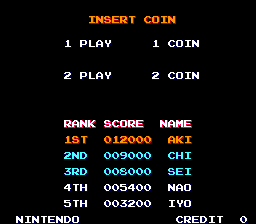
\includegraphics[width=0.25\textwidth]{../img/highscore}};
\end{tikzpicture}
\end{Slide}



\begin{Slide}{Algoritm-exempel: HIGHSCORE}
\Emph{Problem}: Kolla om high-score i ett spel \\ \vspace{1em}

\Emph{Varför?} \pause Så att de som spelar uppmuntras att spela mer :) \\ \vspace{1em}

\Emph{Algoritm:}\pause
\begin{enumerate}
\item $points$ $\leftarrow$ poängen efter senaste spelet
\item $highscore$ $\leftarrow$ bästa resultatet innan senaste spelet
\item \Key{om} $points$ är större än $highscore$ 
\begin{enumerate}[ ~~]
\item  Skriv ''Försök igen!''
\end{enumerate}
\Key{annars}
\begin{enumerate}[ ~~]
\item  Skriv ''Grattis!''
\end{enumerate}
\end{enumerate}
\pause
\scriptsize \Alert{Hittar du buggen?}
\end{Slide}


\begin{Slide}{HIGHSCORE implementerad i Scala}
\begin{Code}
import scala.io.StdIn.readLine

object HighScore {
  def main(args: Array[String]): Unit = {
    val points = readLine("Hur mång poäng fick du?").toInt
    val highscore = readLine("Vad var highscore före senaste spelet?").toInt
    val msg = if (points > highscore) "GRATTIS!" else "Försök igen!"
    println(msg) 
  }
}
\end{Code}
\pause
Är det en bugg eller en feature att det står\\ \texttt{points > highscore} \\ och inte \\ \texttt{points >= highscore} \\ ?
% Buggen är att man inte får GRATTIS om poäng == highscore vilket är tråkigt :)
\end{Slide}


\begin{Slide}{HIGHSCORE implementerad i Java}
\begin{Code}[language=Java]
import java.util.Scanner;

public class HighScore {
    public static void main(String[] args){
        Scanner scan = new Scanner(System.in);
        System.out.println("Hur många poäng fick du?");
        int points =  scan.nextInt();
        System.out.println("Vad var higscore före senaste spelet?");
        int highscore = scan.nextInt();
        if (points > highscore) {
            System.out.println("GRATTIS!");
        } else {
            System.out.println("Försök igen!");
        }
    }
}
\end{Code}
\end{Slide}


\begin{Slide}{Algoritmexempel: N-FAKULTET}
\begin{algorithm}[H]
 \SetKwInOut{Input}{Indata}\SetKwInOut{Output}{Resultat}

 \Input{heltalet $n$}
 \Output{utskrift av produkten av de första $n$ heltalen }
 ~\\
 $prod \leftarrow 1$ \\
 $i \leftarrow 2$  \\
 \While{$i \leq n$}{
  $prod \leftarrow prod * i$\\
  $i \leftarrow i + 1$
 }
 skriv ut $prod$
\end{algorithm}
\pause\vspace{1em}
\begin{itemize}\SlideFontSmall
\item Vad händer om $n$ är noll?
\item Vad händer om $n$ är ett?
\item Vad händer om $n$ är två?
\item Vad händer om $n$ är tre?
\end{itemize}
\end{Slide}

\begin{Slide}{Algoritmexempel: MIN}
\begin{algorithm}[H]
 \SetKwInOut{Input}{Indata}\SetKwInOut{Output}{Resultat}

 \Input{Array $args$ med strängar som alla innehåller heltal}
 \Output{utskrift av minsta heltalet }
 ~\\
 $min \leftarrow$ det största heltalet som kan uppkomma  \\
 $n \leftarrow $ antalet heltal \\
 $i \leftarrow 0$ \\
 \While{$i < n$}{
   $x \leftarrow args(i).toInt$ \\
   \If{( x < $min$)}{$min \leftarrow x$}
   $i \leftarrow i + 1$
 }
 skriv ut $min$
\end{algorithm}
\pause{\hfill \SlideFontTiny \Emph{Test med indata}: \code{args = Array("2", "42", "1", "2")}}
\end{Slide}


\Subsection{Funktioner skapar struktur}

\begin{Slide}{Mall för funktionsdefinitioner}

\code{def} funktionsnamn(parameterdeklarationer): returtyp = block

\pause\vspace{0.5em}\Emph{Exempel}:

\begin{Code}[basicstyle=\ttfamily\fontsize{9}{11}\selectfont]
def öka(i: Int): Int = { i + 1 }
\end{Code}
\pause Om ett enda uttryck: behövs inga \code|{}|. Returtypen kan härledas.
\begin{Code}[basicstyle=\ttfamily\fontsize{9}{11}\selectfont]
def öka(i: Int) = i + 1  
\end{Code}
\pause Om flera parametrar, separera dem med kommatecken: 
\begin{Code}[basicstyle=\ttfamily\fontsize{9}{11}\selectfont]
def isHighscore(points: Int, high: Int): Boolean = {
  val highscore: Boolean = points > high
  if (highscore) println(":)") else print(":(")
  highscore
}
\end{Code}
\pause Ovan funktion har \Alert{sidoeffekten} att skriva ut en smiley.
\end{Slide}

\begin{Slide}{Bättre många små abstraktioner som gör en sak var}

\begin{Code}[basicstyle=\ttfamily\fontsize{8}{11}\selectfont]
def isHighscore(points: Int, high: Int): Boolean = points > high

def printSmiley(isHappy: Boolean): Unit = 
  if (isHappy) println(":)") else print(":(")
\end{Code}

\pause\vspace{2em}
\begin{REPLnonum}
  printSmiley(isHighscore(113,99))
\end{REPLnonum}

\pause\vspace{2em} \code{isHigscore} är en \Emph{äkta funktion} som alltid ger samma svar för samma inparametrar och saknar \Alert{sidoeffekter}.

\end{Slide}



\begin{Slide}{Vad är ett block?}

\begin{itemize}
\item Ett block \Emph{kapslar in} flera satser/uttryck och ser ''utifrån'' ut som en enda sats/uttryck.

\item Ett block skapas med hjälp av klammerparenteser (''krullparenteser'')

\item [] {\fontsize{14}{18}\selectfont \code|{ uttryck1; uttryck2; ... uttryckN }|}\\~

\pause

\item I Scala (till skillnad från många andra språk) har ett block ett \Emph{värde} och är alltså ett \Emph{uttryck}. 

\item Värdet ges av \Emph{sista uttrycket}.

\begin{REPLnonum}
scala> val x = { println(1 + 1); println(2 + 2); 3 + 3 } 
2
4
x: Int = 6
\end{REPLnonum}


\end{itemize}

\end{Slide}

\begin{Slide}{Namn i block blir \textbf{lokala}}
Synlighetsregler: 
\begin{enumerate}
\item Identifierare deklarerade inuti ett block blir \Emph{lokala}.

\item Lokala namn \Alert{överskuggar} namn i yttre block om samma.


\item Namn syns i nästlade underblock.

\end{enumerate}

\begin{REPL}
scala> { val lokaltNamn = 42; println(lokaltNamn) }
42

scala> println(lokaltNamn)
<console>:12: error: not found: value lokaltNamn
       println(lokaltNamn)

scala> { val x = 42; { val x = 76; println(x) }; println(x) }
76
42

scala> { val x = 42; { val y = x + 1; println(y) } }
43
\end{REPL}

\end{Slide}


\begin{Slide}{Parameter och argument}

Skilj på parameter och argument!
\begin{itemize}
\item En \Alert{parameter} är det deklarerade namnet som används \Alert{lokalt} i en funktion för att referera till...

\item \Emph{argumentet} som är värdet som skickas med \Emph{vid anrop} och binds till det lokala parameternamnet.

\end{itemize}


\begin{REPLnonum}
scala> val ettArgument = 42

scala> def öka(minParameter: Int) = minParameter + 1

scala> öka(ettArgument)
\end{REPLnonum}


Speciell syntax: anrop med s.k. \Emph{namngiven parameter}
\begin{REPLnonum}
scala> öka(minParameter = ettArgument) 
\end{REPLnonum}

\end{Slide}

\begin{Slide}{Procedurer}\SlideFontSmall
\begin{itemize}
\item En \Emph{procedur} är en funktion som \Alert{gör} något intressant, men som \Alert{inte} lämnar något intressant returvärde.
\item Exempel på befintlig procedur: \code{println("hej")}
\item Du \Emph{deklarerar egna procedurer} genom att ange \texttt{\Alert{Unit}} som returvärdestyp. Då ges värdet \texttt{\Alert{()}} som betyder ''inget''.
\end{itemize}
\begin{REPL}
scala> def hej(x: String): Unit = println(s"Hej på dej $x!")
hej: (x: String)Unit

scala> hej("Herr Gurka")
Hej på dej Herr Gurka!

scala> val x = hej("Fru Tomat")
Hej på dej Fru Tomat!
x: Unit = ()
\end{REPL}
\begin{itemize}
\item Det som \Alert{görs} kallas (sido)\Emph{effekt}. Ovan är utskriften själva effekten.
\item Funktioner kan också ha sidoeffekter. De kallas då \Alert{oäkta} funktioner.
\end{itemize}
\end{Slide}

\begin{Slide}{''Ingenting'' \emph{är} faktiskt någonting i Scala}
\begin{itemize}
\item I många språk (Java, C, C++, ...) är funktioner som saknar värden speciella.
 Java m.fl. har speciell syntax för procedurer med nyckelordet \jcode{void}, men \Alert{inte} Scala. 

\item I Scala är procedurer inte specialfall; de är vanliga funktioner som returnerar ett värde som \Emph{representerar} ingenting, nämligen () som är av typen Unit. 

\item På så sätt blir procedurer inget undantag utan följer vanlig syntax och semantik precis som för alla andra funktioner.

\item Detta är typiskt för Scala: generalisera koncepten och vi slipper besvärliga undantag! \\(Men vi måste förstå generaliseringen...)


\item [] {\SlideFontSmall 
\url{https://en.wikipedia.org/wiki/Void_type}
\url{https://en.wikipedia.org/wiki/Unit_type}
}

\end{itemize}

\end{Slide}

\begin{Slide}{Abstraktion: Problemlösning genom nedbrytning i enkla funktioner och procedurer som kombineras}\SlideFontSmall
\begin{itemize}
\item En av de allra viktigaste principerna inom programmering är \Emph{funktionell nedbrytning} där  \Emph{underprogram} i form av funktioner och procedurer skapas för att bli byggstenar som kombineras till mer avancerade funktioner och procedurer.

\item Genom de namn som definieras skapas \Emph{återanvändbara abstraktioner} som kapslar in det funktionen gör. 

\item Problemet blir med bra byggblock lättare att lösa.

\item Abstraktioner som beräknar eller gör \Emph{en enda, väldefinierad sak} är enklare att använda, jämfört med de som gör många, helt olika saker.

\item Abstraktioner med \Emph{välgenomtänkta namn} är enklare att använda, jämfört med kryptiska eller missvisande namn.
\end{itemize}

\end{Slide}



\begin{Slide}{Exempel på \textbf{funktionell nedbrytning}}

Kojo-labben gav exempel på \Emph{funktionell nedbrytning} där ett antal abstraktioner skapas och återanvänds.

\begin{Code}
// skapa abstraktioner som bygger på varandra

def kvadrat = upprepa(4){fram; höger}

def stapel = {
  upprepa(10){kvadrat; hoppa}
  hoppa(-10*25)
}

def rutnät = upprepa(10){stapel; höger; fram; vänster}

// huvudprogram 

sudda; sakta(200)
rutnät
\end{Code}
\end{Slide}


\begin{Slide}{Varför abstraktion?}
\begin{itemize}
\item Stora program behöver delas upp annars blir det mycket svårt att förstå och bygga vidare på programmet.
\item Vi behöver kunna välja namn på saker i koden \textit{lokalt}, utan att det krockar med samma namn i andra delar av koden.
\item Abstraktioner hjälper till att hantera och kapsla in komplexa delar så att de blir enklare att använda om och om igen. 

\item Exempel på \Emph{abstraktionsmekanismer} i Scala och Java:
\begin{itemize}

\item \href{https://sv.wikipedia.org/wiki/Klass_\%28programmering\%29}{Klasser} är ''byggblock'' med kod som används för att skapa \href{https://sv.wikipedia.org/wiki/Objektorienterad_programmering\#Objekt}{objekt}, innehållande delar som hör ihop. \\ Nyckelord: \code{class} och \code{object} 

\item \href{https://en.wikipedia.org/wiki/Method_\%28computer_programming\%29}{Metoder} är funktioner som finns i klasser/objekt och används för att lösa specifika uppgifter.  Nyckelord: \code{def}

\item \href{https://en.wikipedia.org/wiki/Java_package}{Paket} används för att organisera kodfiler i en hierarkisk katalogstruktur och skapa namnrymder. \\Nyckelord: \Key{package}

\end{itemize}

\end{itemize}
\end{Slide}


\Subsection{Katalogstruktur för kodfiler med paket}



\begin{Slide}{Källkodsfiler och klassfiler}
\begin{tikzpicture}[node distance=1.5cm]
\node (input) [startstop] {\texttt{Hello.scala}};
\node(inptext) [right of=input, text width=5cm, scale=1.2,xshift=3.5cm]{Källkodsfil};
\node (compile) [process, below of=input] {\texttt{scalac}};
\node (output) [startstop, below of=compile] {\texttt{Hello.class}};
\node(outtext) [right of=output, text width=5cm, scale=1.2,xshift=3.5cm]{\texttt{.class}-fil med byte-kod};
\node (jvm) [process, below of=output] {JVM};
\node(jvmtext) [right of=jvm, text width=5.5cm, scale=0.8,xshift=4.5cm]{\textit{Java Virtual Machine}\\Översätter till maskinkod\\ som passar din specifika CPU\\medan programmet kör};
\draw [arrow] (input) -- (compile);
\draw [arrow] (compile) -- (output);
\draw [arrow] (output) -- (jvm);
\end{tikzpicture}
\end{Slide}




\begin{Slide}{Paket}\SlideFontSmall
\begin{itemize}
\item Paket ger struktur åt kodfilerna. Bra om man har många kodfiler.

\item Byte-koden placeras av kompilatorn i kataloger enligt paketstrukturen.


\end{itemize}

\vspace{1em}
\begin{tikzpicture}[node distance=1.5cm,scale=0.8, every node/.style={transform shape}]
\node (input) [startstop] {\texttt{greeting/Hello.scala}};
\node(inptext) [right of=input, text width=4cm, scale=1.2,xshift=4.5cm]{\lstinline{package greeting}\\\lstinline{object Hello { ... }};
\node (compile) [process, below of=input] {\texttt{scalac  greeting/Hello.java}};
\node (output) [startstop, below of=compile] {\texttt{greeting/Hello.class}};
\node(outtext) [right of=output, text width=4cm, scale=1.2,xshift=4.5cm]{Paketens bytekod hamnar i katalog med samma namn som paketnamnet};
\node (jvm) [process, below of=output] {\texttt{scala greeting.Hello}};
\draw [arrow] (input) -- (compile);
\draw [arrow] (compile) -- (output);
\draw [arrow] (output) -- (jvm);
\end{tikzpicture}

{\SlideFontTiny\vspace{1em} Katalogstrukturen för källkoden måste i Java motsvara paketstrukturen, \\men inte i Scala. Dock kräver många IDE att så görs även för Scala.}
\end{Slide}

\begin{Slide}{Import}
Med hjälp av punktnotation kommer man åt innehåll i ett paket.\\
\begin{Code}
val age = scala.io.StdIn.readLine("Ange din ålder:")
\end{Code}

En \code{import}-sats...
 
\begin{Code}
import scala.io.StdIn.readLine
\end{Code}

...gör så att kompilatorn ''ser'' namnet, och man slipper skriva hela sökvägen till namnet:
\begin{Code}
val age = readLine("Ange din ålder:")
\end{Code}

Man säger att det importerade namnet hamnar \Emph{\textit{in scope}}.
\end{Slide}





\begin{Slide}{Jar-filer}
\texttt{jar}-filer liknar \texttt{zip}-filer och används för att packa ihop bytekod i en enda fil för enkel distribution och körning. 

\vspace{2em}
\begin{tikzpicture}[node distance=1.5cm,scale=0.8, every node/.style={transform shape}]
\node (input) [startstop] {\texttt{greeting/}};
\node(inptext) [right of=input, text width=4cm, scale=1.2,xshift=4.5cm]{en katalog med filer};
\node (jar) [process, below of=input] 
{\texttt{jar cvf minjarfil.jar greeting}};

\node (output) [startstop, below of=compile] {\texttt{minjarfil.jar}};

\node(outtext) [right of=output, text width=4cm, scale=1.2,xshift=4.5cm]{En jar-fil med alla filer inpackade};

\node (jvm) [process, below of=output] {\texttt{scala -cp minjarfil.jar}};

\node(outtextjvm) [right of=jvm, text width=4cm, scale=1.2,xshift=4.5cm]{Lägg jar-filen till \\ ''classpath''};
\draw [arrow] (input) -- (jar);
\draw [arrow] (jar) -- (output);
\draw [arrow] (output) -- (jvm);
\end{tikzpicture}
\end{Slide}

\Subsection{Dokumentation}

\begin{Slide}{Dokumentation}\footnotesize
För att kod ska bli begriplig för människor är det bra att dokumentera vad den gör. Det finns \Emph{tre olika sorters kommentarer} som man kan skriva direkt i Scala/Java-koden, \Alert{som kompilatorn struntar fullständigt i}:
\begin{lstlisting}
// Enradskommentarer börjar med dubbla snedstreck
//       men de gäller bara till radslut

/* Flerradskommentarer börjar med 
   snedstreck-asterisk
   och slutar med asterisk-snedstreck.  */ 

/** Dokumentationskommentarer placeras före 
 *   t.ex. en funktion och berättar vad den gör
 *   och vad eventuella parametrar används till.
 *   Börjar med snedstreck-asterisk-asterisk.
 *   Varje ny kommentarsrad börjar med asterisk.
 *   Avslutas med asterisk-stjärna.
 */
\end{lstlisting}
\end{Slide}

\begin{Slide}{scaladoc}
Programmet \texttt{scaladoc}-filer läser källkod och skapar en webbsajt med dokumentation. 

\vspace{2em}
\begin{tikzpicture}[node distance=1.5cm,scale=0.8, every node/.style={transform shape}]

\node (input) [startstop] {\texttt{greeting/}};

\node(inptext) [right of=input, text width=4cm, scale=1.2,xshift=4.5cm]{en katalog med \texttt{.scala}-filer};

\node (scaladoc) [process, below of=input] 
{\texttt{scaladoc greeting/*.scala}};

\node (output) [startstop, below of=compile] {\texttt{index.html} ~~med mera...};

\node(outtext) [right of=output, text width=4cm, scale=1.2,xshift=4.5cm]{En webbsajt};


\draw [arrow] (input) -- (scaladoc);
\draw [arrow] (scaladoc) -- (output);
\end{tikzpicture}
\end{Slide}



\subsection{Att göra denna vecka}


%%%
\begin{Slide}{Att göra i Vecka \vecka: Förstå grundläggande kodstrukturer}

\begin{enumerate}
\item Laborationer är \Alert{obligatoriska}.\\ Ev. sjukdom måste anmälas \Alert{före} via mejl till kursansvarig!
\item Gör övning \texttt{programs}
\item OBS! Ingen lab denna vecka w02. Använd tiden att komma ikapp om du ligger efter!
\item Träffas i samarbetsgrupper och hjälp varandra att förstå.
\item Vi har nosat på flera koncept som vi kommer tillbaka till senare: du måste inte fatta alla detaljer redan nu.
\item Om ni inte redan gjort det: \\Visa \href{https://github.com/bjornregnell/lth-eda016-2015/tree/master/assignments}{samarbetskontrakt} för handledare på resurstid.
\item \Alert{Koda på resurstiderna} och få hjälp och tips! 
\end{enumerate}
\end{Slide}

\begin{Slide}{Veckans övning: \code{w02-programs}}\SlideFontTiny
\vspace{-0.5em}
\setlength{\leftmargini}{0pt}
\begin{itemize}
%!TEX encoding = UTF-8 Unicode
%!TEX root = ../compendium2.tex

\item Kunna skapa samlingarna Range, Array och Vector med heltals- och strängvärden.
\item Kunna indexera i en indexerbar samling, t.ex. Array och Vector.
\item Kunna anropa operationerna size, mkString, sum, min, max på samlingar som innehåller heltal.
\item Känna till grundläggande skillnader och likheter mellan samlingarna Range, Array och Vector.
\item Förstå skillnaden mellan en for-sats och ett for-uttryck.
\item Kunna skapa samlingar med heltalsvärden som resultat av enkla for-uttryck.
\item Förstå skillnaden mellan en algoritm i pseudo-kod och dess implementation.
\item Kunna implementera algoritmerna SUM, MIN/MAX på en indexerbar samling med en \code{while}-sats.
\item Kunna köra igång enkel Scala-kod i REPL, som skript och som applikation.
\item Kunna skriva och köra igång ett enkelt Java-program.
\item Känna till några grundläggande syntaxskillnader mellan Scala och Java, speciellt variabeldeklarationer och indexering i Array.
\item Förstå vad ett block och en lokal variabel är.
\item Förstå hur nästlade block påverkar namnsynlighet och namnöverskuggning.
\item Förstå kopplingen mellan paketstruktur och kodfilstruktur.
\item Kunna skapa en jar-fil.
\item Kunna skapa dokumentation med scaladoc.

\end{itemize}
\end{Slide}













\Lecture{3}{Funktioner, Objekt}
%!TEX encoding = UTF-8 Unicode
%!TEX root = ../lect-week03.tex


\Subsection{Funktioner}



\begin{Slide}{Deklarera funktioner, överlagring}
\begin{itemize}
\item En parameter, och sedan två parametrar:
\begin{REPL}
scala> :paste
  def öka(a: Int): Int = a + 1
  def öka(a: Int, b: Int) = a + b
  
scala> öka(1)
res0: Int = 2

scala> öka(1,1)
res1: Int = 2

\end{REPL}
\item Båda funktionerna ovan kan finnas samtidigt! Trots att de har samma namn är de \Alert{olika} funktioner; kompilatorn kan skilja dem åt med hjälp av de olika parameterlistorna.

\item Detta kallas \Emph{överlagring} \Eng{overloading} av funktioner.

\end{itemize}
\end{Slide} 


\begin{Slide}{Tom parameterlista och inga parametrar}\SlideFontSmall
\begin{itemize}
\item Om en funktion deklareras med tom parameterlista \code{()} kan den anropas på två sätt: med och utan tomma parenteser.
\begin{REPL}
scala> def tomParameterLista() = 42

scala> tomParameterLista()
res2: Int = 42

scala> tomParameterLista
res3: Int = 42
\end{REPL}

Denna flexibilitet är grunden för \Emph{enhetlig access}: namnet kan användas enhetligt oavsett om det är en funktion eller en variabel.
\item Om parameterlista saknas får man \Alert{inte} använda \code{()} vid anrop:

\begin{REPL}
scala> def ingenParameterLista = 42

scala> ingenParameterLista
res4: Int = 42

scala> ingenParameterLista()
<console>:13: error: Int does not take parameters
       ingenParameterLista()
\end{REPL}

\end{itemize}
\end{Slide} 


\begin{Slide}{Funktioner med defaultargument}\SlideFontSmall

\begin{itemize}
\item Vi kan ofta åstadkomma något som liknar överlagring, men med en enda funktion, om vi i stället använder \Emph{defaultargument}:
\begin{REPLnonum}
scala> def inc(a: Int, b: Int = 1) = a + b
inc: (a: Int, b: Int)Int

scala> inc(42, 2)
res0: Int = 44

scala> inc(42, 1)
res1: Int = 43

scala> inc(42)
res2: Int = 43

\end{REPLnonum}
\item Om argumentet utelämnas och det finns ett defaultargumentet, så är det defaultargumentet som appliceras.
\end{itemize}
\end{Slide} 


\begin{Slide}{Funktioner med namngivna argument}
\begin{itemize}
\item Genom att använda \Emph{namngivna argument} behöver man inte hålla reda på ordningen på parametrarna, bara man känner till parameternamnen. 
\item Namngivna argument går fint att \Alert{kombinera} med defaultargument.
\begin{REPL}
scala> def namn(förnamn: String, 
                efternamn: String, 
                förnamnFörst: Boolean = true,
                ledtext: String = ""): String = 
         if (förnamnFörst) s"$ledtext: $förnamn $efternamn" 
         else s"$ledtext: $efternamn, $förnamn"

scala> namn(ledtext = "Name", efternamn = "Coder", förnamn = "Kim")
res0: String = Name: Kim Coder
\end{REPL}
\end{itemize}
\end{Slide} 


\begin{Slide}{Anropsstacken och objektheapen}\SlideFontSmall
Minnet är uppdelat i två delar:
\begin{itemize}
\item \Emph{Anropsstacken}: På stackminnet läggs en \Emph{aktiveringspost} \Eng{stack frame\footnote{\href{https://en.wikipedia.org/wiki/Call_stack}{en.wikipedia.org/wiki/Call\_stack}}, activation record} för varje funktionsanrop med plats för parametrar och lokala variabler. Aktiveringsposten raderas när returvärdet har levererats. Stacken växer vid nästlade funktionsanrop, då en funktion i sin tur anropar en annan funktion. 

\item \Emph{Objektheapen}: I heapminnet\footnote{\href{https://en.wikipedia.org/wiki/Memory_management}{en.wikipedia.org/wiki/Memory\_management}}$^{,}$\footnote{Ej att förväxlas med datastrukturen heap  \href{https://sv.wikipedia.org/wiki/Heap}{sv.wikipedia.org/wiki/Heap}} sparas alla objekt (data) som allokeras under körning. Heapen städas vid tillfälle av skräpsamlaren \Eng{garbage collector}, och minne som inte används längre frigörs. \\\vspace{0.5em}
\href{http://stackoverflow.com/questions/1565388/increase-heap-size-in-java}{stackoverflow.com/questions/1565388/increase-heap-size-in-java}
\end{itemize}
\end{Slide} 


\begin{Slide}{Aktiveringspost}\SlideFontSmall
Nästlade anrop ger växande anropsstack.
\begin{REPL}
scala> :paste
def f(): Unit = { val n = 5; g(n, 2 * n) }
def g(a: Int, b: Int): Unit = { val x = 1; h(x + 1, a + b) }
def h(x: Int, y: Int): Unit = { val z = x + y; println(z) }

scala> f()

\end{REPL}

\pause
\Alert{Stacken}

\begin{tabular}{|r | l | l |} \hline

variabel & värde & Vilken aktiveringspost? \\ \hline \hline
\pause
 n & 5 & f \\ \hline
 \pause 
 a & 5 & g \\
 b & 10 &  \\
 x & 1  &  \\  \hline
 \pause 
 x & 2  & h \\
 y & 15 &  \\
 z & 17 & \\ \hline
\end{tabular}
\end{Slide} 


\begin{Slide}{Lokala funktioner}\SlideFontSmall
Med lokala funktioner kan delproblem lösas med nästlade abstraktioner. 

\begin{Code}
def gissaTalet(max: Int): Unit = {
  def gissat = io.StdIn.readLine(s"Gissa talet mellan [1, $max]: ").toInt 
  val hemlis = (math.random * max + 1).toInt
  def skrivLedtrådOmEjRätt(gissning: Int): Unit = 
    if (gissning > hemlis) println(s"$gissning är för stort :(") 
    else if (gissning < hemlis) println(s"$gissning är för litet :(")
  def inteRätt(gissning: Int): Boolean = { 
    skrivLedtrådOmEjRätt(gissning)
    gissning != hemlis
  }
  def loop: Int = { var i = 1; while(inteRätt(gissat)){ i += 1 }; i }
  
  println(s"Du hittade talet $hemlis på $loop gissningar :)")
}
\end{Code}

Lokala, nästlade funktionsdeklarationer är tyvärr inte tillåtna i Java.\footnote{\href{http://stackoverflow.com/questions/5388584/does-java-support-inner-local-sub-methods}{\SlideFontSize{8}{9}stackoverflow.com/questions/5388584/does-java-support-inner-local-sub-methods}} 

\end{Slide} 



\begin{Slide}{Värdeanrop och namnanrop}\SlideFontSmall
\begin{itemize}
\item Det vi sett hittills är \Emph{värdeanrop}: argumentet evalueras \Alert{först} innan dess \Alert{värde} \emph{sedan} appliceras:
\begin{REPL}
scala> def byValue(n: Int): Unit = for (i <- 1 to n) print(" " + n)

scala> byValue(21 + 21)
 42 42 42 42 42 42 42 42 42 42 42 42 42 42 42 42 42 42 42 42 42 42 42 42 42 42 42 42 42 42 42 42 42 42 42 42 42 42 42 42 42 42

scala> byValue({print(" hej"); 21 + 21})
 hej 42 42 42 42 42 42 42 42 42 42 42 42 42 42 42 42 42 42 42 42 42 42 42 42 42 42 42 42 42 42 42 42 42 42 42 42 42 42 42 42 42 42
\end{REPL}
\item Men man kan med \code{=>} före parametertypen åstadkomma \Emph{namnanrop}: argumentet \Alert{''klistras in''} i stället för \Alert{namnet} och evalueras \Alert{varje gång} (kallas även \Emph{fördröjd evaluering}):
\begin{REPL}
scala> def byName(n: => Int): Unit = for (i <- 1 to n) print(" " + n)

scala> byName({print(" hej"); 21 + 21})
 hej hej 42 hej 42 hej 42 hej 42 hej 42 hej 42 hej 42 hej 42 hej 42 hej 42 hej 42 hej 42 hej 42 hej 42 hej 42 hej 42 hej 42 hej 42 hej 42 hej 42 hej 42 hej 42 hej 42 hej 42 hej 42 hej 42 hej 42 hej 42 hej 42 hej 42 hej 42 hej 42 hej 42 hej 42 hej 42 hej 42 hej 42 hej 42 hej 42 hej 42 hej 42 hej 42
\end{REPL}

\end{itemize}
\end{Slide} 

\begin{Slide}{Klammerparenteser vid ensam parameter}
Så här har vi sett nyss att man man göra:
\begin{REPL}
scala> def loop(n: => Int): Unit = for (i <- 1 to n) print(" " + n)

scala> loop(21 + 21)

scala> loop({print(" hej"); 21 + 21})
\end{REPL}

Men...\\För alla funktioner \code{f} gäller att: \\ det är helt ok att byta ut vanliga parenteser: \hfill\code{f(uttryck)} \\ mot krullparenteser: \hfill\code|f{uttryck}| \\ \Alert{om} parameterlistan har \Alert{exakt en} parameter.  

\vspace{0.5em}Men man kan alltså göra så här också:
\begin{REPLnonum}
scala> loop{ 21 + 21 }

scala> loop{ print(" hej"); 21 + 21 }
\end{REPLnonum}


\end{Slide} 

\begin{Slide}{Uppdelad parameterlista}
\begin{itemize}
\item Vi har tidigare sett att man kan ha mer än en parameter:
\begin{REPLnonum}
scala> def add(a: Int, b: Int) = a + b

scala> add(21, 21)
res0: Int = 42
\end{REPLnonum}

\item Man kan även ha \Alert{mer än en} parameterlista:
\begin{REPLnonum}

scala> def add(a: Int)(b: Int) = a + b

scala> add(21)(21)
res1: Int = 42
\end{REPLnonum}
\item Detta kallas även \Emph{multipla parameterlistor} \Eng{multiple parameter lists}
\end{itemize}
\href{http://docs.scala-lang.org/style/declarations.html#multiple-parameter-lists}{\SlideFontTiny docs.scala-lang.org/style/declarations.html\#multiple-parameter-lists}
\end{Slide} 


\begin{Slide}{Skapa din egen kontrollstruktur}
\begin{itemize}
\item Genom att \Alert{kombinera} \Emph{uppdelad parameterlista} med \Emph{namnanrop} med \Emph{klammerparentes vid ensam parameter} kan vi skapa vår egen kontrollstruktur:
\begin{REPLnonum}
scala> def upprepa(n: Int)(block: => Unit) = { 
         var i = 0
         while (i < n) { block; i += 1 }
       }

scala> upprepa(42){ 
         if (math.random < 0.5) {
           print(" gurka")
         } else {
           print(" tomat")
         }
       }
 gurka gurka gurka tomat tomat gurka gurka gurka gurka tomat tomat tomat tomat tomat gurka tomat tomat tomat tomat tomat tomat tomat tomat tomat gurka gurka gurka tomat tomat gurka gurka gurka tomat tomat gurka tomat gurka gurka gurka gurka tomat tomat
\end{REPLnonum}
\end{itemize}
\end{Slide} 


\begin{Slide}{Funktioner är äkta värden i Scala}\SlideFontSmall
\begin{itemize}
\item En funktioner är ett äkta värde.
\item Vi kan till exempel tilldela en variabel ett funktionsvärde. 
\item Med hjälp av blank+understreck efter funktionsnamnet får vi funktionen som ett \Alert{värde} (inga argument appliceras än):
\begin{REPLnonum}
scala> def add(a: Int, b: Int) = a + b

scala> val f = add _

scala> f
f: (Int, Int) => Int = <function2>

scala> f(21, 21)
res0: Int = 42
\end{REPLnonum}

\item Ett funktionsvärde har en \Alert{typ} precis som alla värden: \\ 
\code{f: (Int, Int) => Int}
\end{itemize}
\end{Slide} 

\begin{Slide}{Funktionsvärden kan vara argument}
\begin{itemize}
\item En funktion kan ha en annan funktion som parameter:
\begin{REPL}
scala> def tvåGånger(x: Int, f: Int => Int) = f(f(x))

scala> def öka(x: Int) = x + 1

scala> def minska(x: Int) = x - 1

scala> tvåGånger(42, öka _)
res1: Int = 43

scala> tvåGånger(42, minska _)
res1: Int = 41
\end{REPL}

\item Om argumentets funktionstyp \Alert{kan härledas} av kompilatorn och \Alert{passar} med parametertypen så behövs ej understreck: \\ 
\begin{REPL}
scala> tvåGånger(42, öka)
res1: Int = 43
\end{REPL}\end{itemize}
\end{Slide}



\begin{Slide}{Applicera funktioner på element i samlingar med \texttt{map}}\SlideFontSmall
\begin{REPL}
scala> def öka(x: Int) = x + 1

scala> def minska(x: Int) = x - 1

scala> val xs = Vector(1, 2, 3)

scala> xs.map(öka)
res0: scala.collection.immutable.Vector[Int] = Vector(2, 3, 4)

scala> xs.map(minska)
res1: scala.collection.immutable.Vector[Int] = Vector(0, 1, 2)

scala> xs map öka
res2: scala.collection.immutable.Vector[Int] = Vector(2, 3, 4)

scala> xs map minska
res3: scala.collection.immutable.Vector[Int] = Vector(0, 1, 2)
\end{REPL}
Funktioner som tar andra funktioner som parametrar kallas \\ \Emph{högre ordningens funktioner}. 
\end{Slide} 




\begin{Slide}{Anonyma funktioner}
\begin{itemize}
\item  Man behöver inte ge funktioner namn. De kan i stället skapas med hjälp av \Emph{funktionsliteraler}.\footnote{Även kallat ''lambda-värde'' eller bara ''lamda'' efter den s.k. lambdakalkylen. \href{https://en.wikipedia.org/wiki/Anonymous_function}{en.wikipedia.org/wiki/Anonymous\_function}}

\item En funktionsliteral har ...
\begin{enumerate}
\item en parameterlista (utan funktionsnamn) och ev. returtyp, \item sedan den reserverade teckenkombinationen \code{=>} \item och sedan ett uttryck (eller ett block).
\end{enumerate}
\item Exempel:
\begin{Code}[basicstyle=\ttfamily\fontsize{10}{12}\selectfont]
(x: Int, y: Int): Int => x + y
\end{Code}
\pause
\item Om kompilatorn kan gissa typerna från sammanhanget så behöver typerna inte anges i själva  funktionsliteralen:
\begin{Code}[basicstyle=\ttfamily\fontsize{10}{12}\selectfont]
val f: (Int, Int) => Int = (x, y) => x + y
\end{Code}

\end{itemize}
\end{Slide}


\begin{Slide}{Applicera anonyma funktioner på element i samlingar}\SlideFontSmall
\begin{itemize}
\item Anonym funktion skapad med funktionsliteral direkt i anropet:
\begin{REPL}
scala> val xs = Vector(1, 2, 3)

scala> xs.map((x: Int): Int => x + 1)
res0: scala.collection.immutable.Vector[Int] = Vector(2, 3, 4)
\end{REPL}
\item Eftersom kompilatorn här kan härleda typerna så behövs de inte:
\begin{REPL}
scala> xs.map(x => x - 1)
res1: scala.collection.immutable.Vector[Int] = Vector(0, 1, 2)

scala> xs map (x => x - 1)
res2: scala.collection.immutable.Vector[Int] = Vector(0, 1, 2)

\end{REPL}
\item Om man bara använder parametern en enda gång i funktionen så kan man byta ut parameternamnet mot ett understreck.

\begin{REPL}
scala> xs.map(_ + 1)
res3: scala.collection.immutable.Vector[Int] = Vector(2, 3, 4)
\end{REPL}
\end{itemize}
\end{Slide} 



\begin{Slide}{Platshållarsyntax för anonyma funktioner}\SlideFontSmall
\begin{itemize}
\item Understreck i funktionsliteraler kallas \Emph{platshållare} \Eng{placeholder} och medger ett förkortat skrivsätt \Alert{om} den parameter som understrecket representerar används \Alert{endast en gång}.

\begin{Code}[basicstyle=\ttfamily\fontsize{10}{12}\selectfont]
_ + 1
\end{Code}
Ovan expanderas av kompilatorn till följande funktionsliteral \\(där namnet på parametern är godtyckligt):
\begin{Code}[basicstyle=\ttfamily\fontsize{10}{12}\selectfont]
x => x + 1
\end{Code}
\pause
\item Det kan förekomma flera understreck; det första avser första parametern, det andra avser andra parametern etc.
\begin{Code}[basicstyle=\ttfamily\fontsize{10}{12}\selectfont]
_ + _
\end{Code}
... expanderas till:
\begin{Code}[basicstyle=\ttfamily\fontsize{10}{12}\selectfont]
(x, y) => x + y 
\end{Code}

\end{itemize}
\end{Slide} 


\begin{Slide}{Exempel på platshållarsyntax med samlingsmetoden \texttt{reduceLeft}}\SlideFontSmall
Metoden \code{reduceLeft} applerar en funktion på de två första elementen och tar sedan på resultatet som första argument och nästa element som andra argument och upprepar detta genom hela samlingen. 
\begin{REPL}
scala> def summa(x: Int, y: Int) = x + y

scala> val xs = Vector(1, 2, 3, 4, 5)

scala> xs.reduceLeft(summa)
res20: Int = 15

scala> xs.reduceLeft((x, y) => x + y)
res21: Int = 15

scala> xs.reduceLeft(_ + _)
res22: Int = 15

scala> xs.reduceLeft(_ * _)
res23: Int = 120
\end{REPL}
\end{Slide} 


\begin{Slide}{Stegade funktioner, ''Curry-funktioner''}
Om en funktion har en uppdelad parameterlista kan man skapa \Emph{stegade funktioner}, även kallat \Emph{partiellt applicerade} funktioner \Eng{partially applied functions} eller \Emph{''Curry''-funktioner}.
\begin{REPLnonum}
scala> def add(x: Int)(y: Int) = x + y  

scala> val öka = add(1) _
öka: Int => Int = <function1>

scala> Vector(1,2,3).map(öka)
res0:scala.collection.immutable.Vector[Int]= Vector(2, 3, 4)

scala> Vector(1,2,3).map(add(2))
res1:scala.collection.immutable.Vector[Int]= Vector(3, 4, 5)
\end{REPLnonum}
\end{Slide} 

\begin{Slide}{Översikt begrepp vi gått igenom hittills}
\begin{itemize}
\item överlagring
\item utelämna tom parameterlista (enhetlig access)
\item defaultargument
\item namngivna argument
\item lokala funktioner
\item namnanrop (fördröjd evaluering)
\item klammerparentes vid ensam paramenter
\item uppdelad parameterlista
\item egendefinierade kontrollstrukturer
\item funktioner som äkta värden
\item anonyma funktioner
\item stegade funktioner (''Curry-funktioner'')
\end{itemize}
\end{Slide} 

\begin{Slide}{Begränsningar i Java}\SlideFontTiny
\begin{itemize}
\item Av alla dessa funktionskoncept...
\begin{itemize}\SlideFontTiny
\item överlagring
\item utelämna tom parameterlista (principen om enhetlig access)
\item defaultargument
\item namngivna argument
\item lokala funktioner
\item namnanrop (fördröjd evaluering)
\item klammerparentes vid ensam paramenter
\item uppdelad parameterlista
\item egendefinierade kontrollstrukturer
\item funktioner som äkta värden
\item anonyma funktioner
\item stegade funktioner (''Curry-funktioner'')
\end{itemize}
\item ...kan man endast göra \Emph{överlagring} i Java 7, 
\item medan även \Emph{anonyma funktioner} (''lambda'') går att göra (med vissa begränsningar) i Java 8. \href{https://en.wikipedia.org/wiki/Anonymous_function\#Java_Limitations}{en.wikipedia.org/wiki/Anonymous\_function\#Java\_Limitations}
\item \vspace{0.5em} En av de saker jag saknar mest i Java: \Alert{lokala funktioner}!
\end{itemize}
Det är \Alert{kombinationen} av alla koncept som \Alert{skapar uttryckskraften} i Scala.

\end{Slide} 





%!TEX encoding = UTF-8 Unicode
%!TEX root = ../lect-week03.tex

\Subsection{Objekt}

\begin{Slide}{Objekt som modul}
\begin{itemize}
\item Ett \code{object} användas ofta för att samla \Emph{medlemmar} \Eng{members} som \Alert{hör ihop} och ge dem en egen \Emph{namnrymd} \Eng{name space}. 
\item Medlemmarna kan vara t.ex.: 
\begin{itemize}
\item  \code{val} \item \code{var} \item \code{def} 
\end{itemize}
\item Ett sådant objekt kallas även för \Emph{modul}.\footnote{
Även paket som skapas med \code{package} har en egen namnrymd och är därmed också en slags modul. Objekt kan alltså i Scala användas som ett alternativ till paket; en skillnad är att objekt kan ha tillstånd och att objekt inte skapar underkataloger vid kompilering (det finns iofs s.k. \code{package object}) \href{https://en.wikipedia.org/wiki/Modular_programming}{en.wikipedia.org/wiki/Modular\_programming}}

\end{itemize}

\end{Slide}

\begin{Slide}{Singelobjekt och metod} \SlideFontSmall
Ett Scala-\code{object} är ett s.k. \Emph{singelobjekt} \Eng{singleton object} och finns bara i \Alert{en} enda upplaga. \\ Minne för objektets variabler allokeras första gången objektet refereras. \\ En funktion som finns i ett objekt kallas en \Emph{metod} \Eng{method}.
\begin{Code}[basicstyle=\ttfamily\fontsize{9}{11}\selectfont]
object mittBankkonto {
  val kontonr: Long        = 1234567L
  var saldo: Int           = 1000
  def ärSkuldsatt: Boolean = saldo < 0
}
\end{Code}
\begin{REPLnonum}
scala> mittBankkonto.saldo -= 25000

scala> mittBankkonto.ärSkuldsatt
res0: Boolean = true
\end{REPLnonum}

(Vi ska i nästa vecka se hur man med s.k. klasser kan skapa många upplagor av samma  typ av objekt, så att vi kan ha flera olika bankkonto.)
\end{Slide} 



\begin{Slide}{Vad är ett tillstånd?} 
Ett objekts \Emph{tillstånd} är den samlade uppsättningen av värden av alla de variabler som finns i objektet.
\begin{Code}[basicstyle=\ttfamily\fontsize{9}{11}\selectfont]
object mittBankkonto {
  val kontonr: Long        = 1234567L
  var saldo: Int           = 1000
  def ärSkuldsatt: Boolean = saldo < 0
}
\end{Code}
\begin{tikzpicture}[font=\large\sffamily]
\matrix [matrix of nodes, row sep=0, column 2/.style={nodes={rectangle,draw,minimum width=0.8cm}}] (mat) 
{
\texttt{mittBankkonto}   &  \makebox(10,10){ }\\
%\texttt{g2}   &  \makebox(16,12){ }\\
};
\node[cloud, cloud puffs=13.0, cloud ignores aspect, minimum width=2cm, minimum height=3.8cm,
 align=center, draw] (x) at (5.8cm, -1.5cm) {
 \begin{tabular}{r l}
 \texttt{kontonr} & \fbox{1234567L} \\
 \texttt{saldo} & \fbox{1000}\\
 \end{tabular}
 };
\filldraw[black] (1.7cm,0.0cm) circle (3pt) node[] (ref) {};
 \draw [arrow, line width=0.7mm] (ref) -- (x);
% \node[cloud, cloud puffs=15.7, cloud ignores aspect, %minimum width=5cm, minimum height=2cm,
% align=center, draw] (g2) at (5cm, -2cm) {Gurka-\\objekt};
% \filldraw[black] (0.4cm,-0.4cm) circle (3pt) node[] (g2ref) {};
% \draw [arrow] (g2ref) -- (g2);
\end{tikzpicture}
\end{Slide} 


\begin{Slide}{Tillståndsändring} 

När en variabel tilldelas ett nytt värde sker en \Emph{tillståndsändring}. Ett \Emph{förändringsbart objekt} \Eng{mutable object} har ett \Emph{förändringsbart tillstånd} \Eng{mutable state}. 

\begin{REPLnonum}
scala> mittBankkonto.saldo -= 25000

scala> bankKonto.saldo
res1: Int = -24000
\end{REPLnonum}
\begin{tikzpicture}[font=\large\sffamily]
\matrix [matrix of nodes, row sep=0, column 2/.style={nodes={rectangle,draw,minimum width=0.8cm}}] (mat) 
{
\texttt{mittBankkonto}   &  \makebox(10,10){ }\\
%\texttt{g2}   &  \makebox(16,12){ }\\
};
\node[cloud, cloud puffs=13.0, cloud ignores aspect, minimum width=2cm, minimum height=3.8cm,
 align=center, draw] (x) at (5.8cm, -1.5cm) {
 \begin{tabular}{r l}
 \texttt{kontonr} & \fbox{1234567L} \\
 \texttt{saldo} & \fbox{-24000}\\
 \end{tabular}
 };
\filldraw[black] (1.7cm,0.0cm) circle (3pt) node[] (ref) {};
 \draw [arrow, line width=0.7mm] (ref) -- (x);
% \node[cloud, cloud puffs=15.7, cloud ignores aspect, %minimum width=5cm, minimum height=2cm,
% align=center, draw] (g2) at (5cm, -2cm) {Gurka-\\objekt};
% \filldraw[black] (0.4cm,-0.4cm) circle (3pt) node[] (g2ref) {};
% \draw [arrow] (g2ref) -- (g2);
\end{tikzpicture}
\end{Slide} 

\begin{Slide}{Vad rymmer sköldpaddan i Kojo i sitt tillstånd?} 
\begin{figure}
\centering
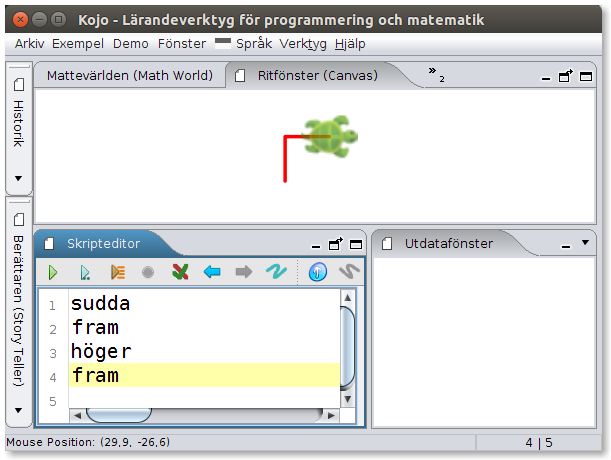
\includegraphics[width=0.7\textwidth]{../img/kojo}
\end{figure}
\pause position, rikting, pennfärg, pennbredd, penna uppe/nere, fyllfärg
\end{Slide} 

\begin{Slide}{Lata variabler och fördröjd evaluering} 
Med nyckelordet \code{lazy} före \code{val} skapas en s.k. ''lat'' \Eng{lazy} variabel.
\begin{REPL}
scala> val striktVektor = Vector.fill(1000000)(math.random)
striktVektor: scala.collection.immutable.Vector[Double] = 
 Vector(0.7583305221813246, 0.9016192590993339, 0.770022134260162, 0.15667718184929746, ...
 
scala> lazy val latVektor = Vector.fill(1000000)(math.random)
latVektor: scala.collection.immutable.Vector[Double] = <lazy>

scala> latVektor
res0: scala.collection.immutable.Vector[Double] = 
  Vector(0.5391685014341797, 0.14759775960530275, 0.722606095900537, 0.9025572787055386, ... 
\end{REPL}

En \code {lazy val} initialiseras \Alert{inte} vid deklarationen utan när den \Alert{refereras första gången}. Yttrycket som anges i deklarationen evalueras med s.k. \Emph{fördröjd evaluering} (även ''lat'' evaluering). 
\end{Slide} 

\begin{Slide}{Vad är egentligen skillnaden mellan \texttt{val}, \texttt{var}, \texttt{def} och \texttt{lazy val}?} 
\begin{Code}[basicstyle=\ttfamily\fontsize{8}{11}\selectfont]
object slump {
  val förAlltidSammaReferens  = math.random
  var kanÄndrasMedTilldelning = math.random
  def evaluerasVidVarjeAnrop  = math.random
  lazy val fördröjdInit       = Vector.fill(1000000)(math.random)
}
\end{Code}
\vspace{1em}\pause
Lat evaluering är en viktig princip inom funktionsprogrammering som möjliggör effektiva, oföränderliga datastrukturer där element allokeras först när de behövs. \\
\href{https://en.wikipedia.org/wiki/Lazy_evaluation}{en.wikipedia.org/wiki/Lazy\_evaluation}
\end{Slide} 


\Subsection{Funktioner är objekt}

\begin{Slide}{Programmeringsparadigm}
\href{https://en.wikipedia.org/wiki/Programming_paradigm}{en.wikipedia.org/wiki/Programming\_paradigm}:
\begin{itemize}
\item \Emph{Imperativ programmering}: programmet är uppbyggt av sekvenser av olika satser som läser och \Alert{ändrar} tillstånd
\item \Emph{Objektorienterad programmering}: en sorts imperativ programmering där programmet består av objekt som kapslar in tillstånd och erbjuder operationer som läser och \Alert{ändrar} tillstånd.
\item \Emph{Funktionsprogrammering}: programmet är uppbyggt av samverkande (matematiska) funktioner som \Alert{undviker} föränderlig data och tillståndsändringar. Oföränderliga datastrukturer skapar effektiva program i kombination med lat evaluering och rekursion. 
\end{itemize}
\end{Slide} 


\begin{Slide}{Funktioner är äkta objekt i Scala}
Scala visar hur man kan \Alert{förena} \Eng{unify} \\ \Emph{objekt-orientering} och \Emph{funktionsprogrammering}: \\\vspace{0.5em}

\textbf{\Large En funktion är ett objekt av funktionstyp\\ som har en \code{apply}-metod.}
\pause
\begin{REPLnonum}
scala> object öka extends (Int => Int) { 
         def apply(x: Int) = x + 1 
       }


scala> öka(1)
res0: Int = 2

scala> öka.   // tryck TAB
andThen   apply   compose   toString
\end{REPLnonum}
Mer om \code{extends} senare i kursen... %extends (Int => Int skrivs om till Function1[Int, Int]
\end{Slide} 


\Subsection{Rekursion}
\begin{Slide}{Rekursiva funktioner}
\begin{itemize}
\item Funktioner som \Alert{anropar sig själv} kallas \Emph{rekursiva}.


\begin{REPLnonum}
scala> def fakultet(n: Int): Int = 
         if (n < 2) 1 else n * fakultet(n - 1)

scala> fakultet(5)
res0: Int = 120
\end{REPLnonum}

\item För varje nytt anrop läggs en ny aktiveringspost på stacken. 

\item I aktiveringsposten sparas varje returvärde som gör att \code{5 * (4 * (3 * (2 * 1)))} kan beräknas. 

\item Rekrusionen avbryts när man når \Emph{basfallet}, här \code{n < 0}

\item En rekursiv funktion \Alert{måste} ha en returtyp.

\end{itemize}

\end{Slide} 

\begin{Slide}{Loopa med rekursion}
\begin{Code}
def gissaTalet(max: Int): Unit = {
  def gissat = io.StdIn.readLine(s"Gissa talet mellan [1, $max]: ").toInt 
  val hemlis = (math.random * max + 1).toInt
  def skrivLedtrådOmEjRätt(gissning: Int): Unit = 
    if (gissning > hemlis) println(s"$gissning är för stort :(") 
    else if (gissning < hemlis) println(s"$gissning är för litet :(")
  def ärRätt(gissning: Int): Boolean = { 
    skrivLedtrådOmEjRätt(gissning)
    gissning == hemlis
  }
  def loop(n: Int = 1): Int = if (ärRätt(gissat)) n else loop(n + 1)
  
  println(s"Du hittade talet $hemlis på ${loop()} gissningar :)")
}
\end{Code}
\end{Slide} 


\begin{Slide}{Rekursiva datastrukturer}

\begin{itemize}
\item Datastrukturena Lista och Träd är exempel på datastrukturer som passar bra ihop med rekursion. 
\item Båda dessa datastrukturer kan beskrivas rekursivt:
\begin{itemize}
\item En lista består av ett huvud och en lista, som i sin tur består av ett huvud och en lista, som i sin tur...
\item Ett träd består av grenar till träd som i sin tur består av grenar till träd som i sin tur, ...
\end{itemize}
\item Dessa datastrukturer bearbetas med fördel med rekursiva algoritmer.
\item I denna kursen ingår rekursion endast ''för kännedom'': \\ du ska veta vad det är och kunna skapa en enkel rekursiv funktion, t.ex. fakultets-beräkning. Du kommer jobba mer med rekursion och rekursiva datastrukturer i fortsättningskursen.
\end{itemize}
\end{Slide} 

\Subsection{SimpleWindow}
\begin{Slide}{Färdiga, enkla funktioner för att rita finns i klassen \texttt{cslib.window.SimpleWindow}}
På labben ska du använda \code{cslib.window.SimpleWindow}
\begin{itemize}
\item Paketet \code{cslib} innehåller paketet \code{window} som innehåller Java-klassen \code{SimpleWindow}.
%\item En \Emph{klass} är en ''mall'' för att göra \Emph{objekt}. 
\item Med \code{SimpleWindow} kan man skapa ritfönster. 
%\item När man skapar ett objekt från en klass använder man nyckelordet \code{new}.
\item Ladda ner \url{http://cs.lth.se/pgk/cslib} och lägg sedan jar-filen den katalog där du startar REPL med: \code{scala -cp cslib.jar}
\end{itemize}
\pause
\begin{REPLnonum}
$ scala -cp cslib.jar
scala> val w = new SimpleWindow(200,200,"hejsan")  
\end{REPLnonum}
\pause Studera dokumentationen för \code{cslib.window.SimpleWindow} här: \url{http://cs.lth.se/pgk/api/}
\end{Slide} 



\Subsection{Veckans övning och laboration}


\begin{Slide}{Övning \texttt{functions}}\SlideFontTiny
\setlength{\leftmargini}{0pt}
\begin{itemize}
%!TEX encoding = UTF-8 Unicode
%!TEX root = ../compendium2.tex

\item Kunna skapa och använda funktioner med en eller flera parametrar, default-argument, namngivna argument, och uppdelad parameterlista.
\item Kunna använda funktioner som äkta värden.
\item Kunna skapa och använda anonyma funktioner (s.k. lambda-funktioner).
\item Kunna applicera en funktion på element i en samling.
\item Förstå skillnader och likheter mellan en funktion och en procedur.
\item Förstå skillnader och likheter mellan en värde-anrop och namnanrop.
\item Kunna skapa en procedur i form av en enkel kontrollstruktur med fördröjd evaluering av ett block.
\item Kunna skapa och använda objekt som moduler.
\item Förstå skillnaden mellan äkta funktioner och funktioner med sidoeffekter.
\item Kunna skapa och använda variabler med fördröjd initialisering och förstå när de är användbara.
\item Kunna förklara hur nästlade funktionsanrop fungerar med hjälp av begreppet aktiveringspost.
\item Kunna skapa och använda lokala funktioner, samt förstå nyttan med lokala funktioner.
\item Känna till att funktioner är objekt med en \code{apply}-metod.
\item Känna till stegade funktioner och kunna använda partiellt applicerade argument.
\item Känna till rekursion och kunna förklara hur rekursiva funktioner fungerar.
%\item Känna till svansrekursion och att svansrekursiva funktioner kan optimeras till loopar.

\end{itemize}
\end{Slide} 


\begin{Slide}{Lab \texttt{blockmole}}%\SlideFontTiny
%\setlength{\leftmargini}{0pt}
\begin{itemize}
%!TEX encoding = UTF-8 Unicode
%!TEX root = ../compendium.tex

\item Kunna kompilera Scalaprogram med \texttt{scalac}.
\item Kunna köra Scalaprogram med \texttt{scala}.
\item Kunna definiera och anropa funktioner.
\item Kunna använda och förstå default-argument.
\item Kunna ange argument med parameternamn.
\item Kunna definiera objekt med medlemmar.
\item Förstå kvalificerade namn och import.
\item Förstå synlighet och skuggning.

\end{itemize}

\end{Slide} 



\Lecture{4}{Datastrukturer}
%!TEX encoding = UTF-8 Unicode
%!TEX root = ../lect-week04.tex

\ifkompendium\else

\begin{Slide}{Denna vecka: Fatta datastrukturer}
\begin{itemize}
\item Läs teori
\item Gör övning \code{data}
\item Gör lab \code{???}
\end{itemize}
\end{Slide}

\fi

%%%

\begin{Slide}{Olika sätt att skapa datastrukturer}
\begin{itemize}
\item Tupler
  \begin{itemize}
  \item samla $n$ st datavärden i element \Emph{\code{_1}}, \Emph{\code{_2}}, ...  \code{_}$n$
  \item elementen kan vara av \Alert{olika} typ
  \end{itemize}
\item Klasser   
  \begin{itemize}
  \item samlar data i \Emph{attribut} med (väl valda!) namn
  \item attributen kan vara av \Alert{olika} typ
  \item definierar även metoder som använder attributen (operationer på data)
  \end{itemize}

\item Samlingar 
  \begin{itemize}
  \item speciella klasser som samlar data i element av \Alert{samma} typ
  \item finns ofta \emph{många} färdiga \Emph{bra-att-ha-metoder} 
  \end{itemize}
\end{itemize}
\end{Slide}

\ifkompendium\else

\begin{Slide}{Vad är en tupel?}
\code{("hej", 42, math.Pi)} är en 3-tupel med typ: \code{(String, Int, Double)}
\end{Slide}

\fi


\begin{Slide}{Hierarki av samlingar i scala.collection}
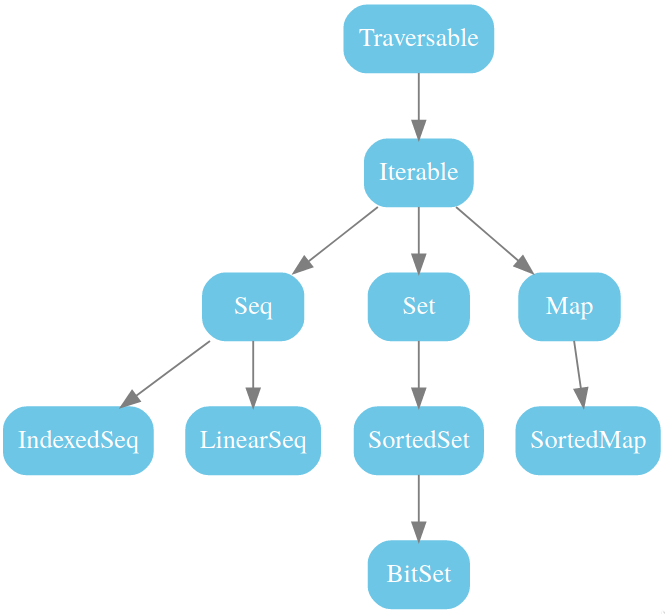
\includegraphics[width=1.0\textwidth]{../img/collection/collection-traits}
\end{Slide}

\ifkompendium
\noindent Läs mer om Scalas samlingar här: \\ 
\url{http://docs.scala-lang.org/overviews/collections/overview}
\else\fi

\ifkompendium\else

\begin{Slide}{scala.collection.immutable}
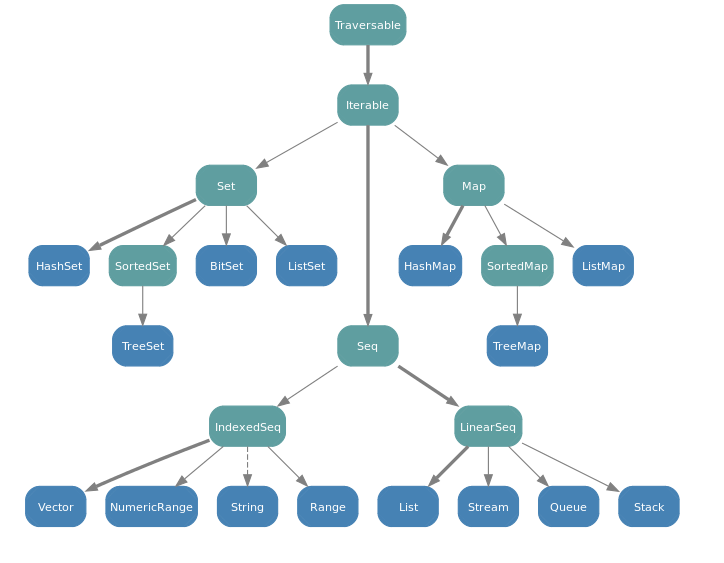
\includegraphics[width=0.82\textwidth]{../img/collection/collection-immutable}
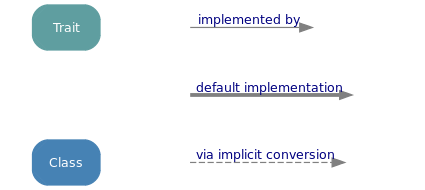
\includegraphics[width=0.33\textwidth]{../img/collection/collection-legend}
\end{Slide}

\begin{Slide}{scala.collection.mutable}
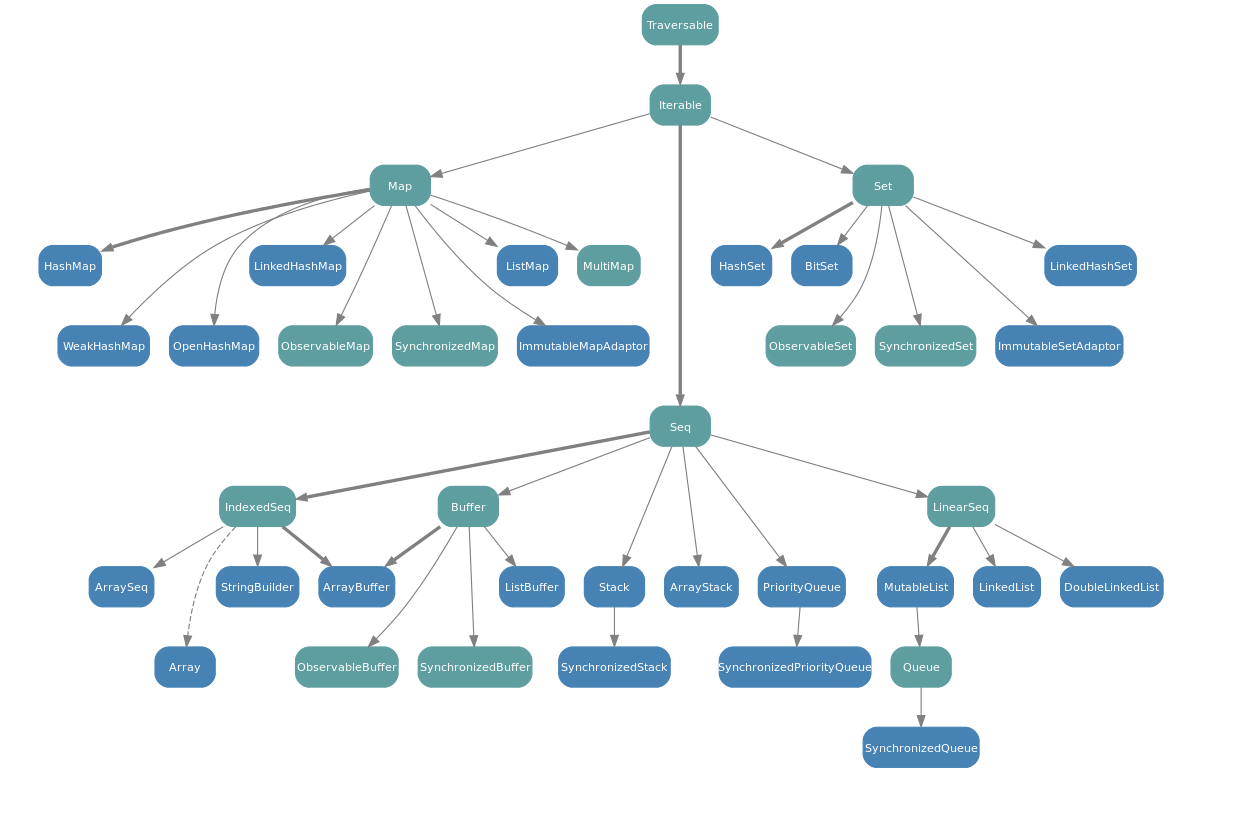
\includegraphics[width=1.05\textwidth]{../img/collection/collection-mutable}
\end{Slide}
\fi


% ??? Berätta om javafx.util.pair
% http://stackoverflow.com/questions/521171/a-java-collection-of-value-pairs-tuples




%!TEX encoding = UTF-8 Unicode
%!TEX root = ../lect-week04.tex

\ifkompendium\else

\Subsection{Tupler}

\begin{Slide}{Vad är en tupel?}\SlideFontSmall

\begin{itemize}
\item En tupel samlar $n$ st objekt i en enkel struktur, med koncis syntax.
  \item Elementen kan vara av \Alert{olika} typ.

\item 
\code{("hej", 42, math.Pi)} är en \Emph{3-tupel} av typen: \code{(String, Int, Double)}

\item Du kan komma åt de enskilda elementen med \Emph{\code{_1}}, \Emph{\code{_2}}, ...  \code{_}$n$

\begin{REPL}
scala> val t = ("hej", 42, math.Pi)
t: (String, Int, Double) = (hej,42,3.141592653589793)

scala> t._1
res0: String = hej

scala> t._2
res1: Int = 42
\end{REPL}

\item Tupler är praktiska när man inte vill ta det lite större arbetet att skapa en egen klass.
(Men med klasser kan man göra mycket mer än med tupler.)

\item I Scala kan du skapa tupler upp till en storlek av 22 element. 
\\ (Behöver du fler element, använd i stället en samling, t.ex. \code{Vector}.)

\end{itemize}

\end{Slide}




\begin{Slide}{Tupler som parametrar och returvärde.}\SlideFontSmall

\begin{itemize}

\item Tupler är smidiga när man på ett enkelt och typsäkert sätt vill låta en funktion \Emph{returnera mer än ett värde}.

\begin{REPL}
scala> def längd(p: (Double, Double)) = math.hypot(p._1, p._2)

scala> def vinkel(p: (Double, Double)) = math.atan2(p._1, p._2) 

scala> def polär(p: (Double, Double)) = (längd(p), vinkel(p))

scala> polär((3,4))
res2: (Double, Double) = (5.0,0.6435011087932844)

\end{REPL}
\vspace{0.5em}
\item Om typerna passar kan man skippa dubbla parenteser vid \Emph{ensamt tupel-argument}:
\begin{REPL}
scala> polär(3,4)
res3: (Double, Double) = (5.0,0.6435011087932844)
\end{REPL}
\item[] {\SlideFontTiny\href{https://sv.wikipedia.org/wiki/Pol\%C3\%A4ra_koordinater}{https://sv.wikipedia.org/wiki/Polära\_koordinater}}


\end{itemize}
\end{Slide}

\begin{Slide}{Ett smidigt sätt att skapa 2-tupler med metoden \texttt{->}}
Det finns en metod vid namn \code{->} som kan användas på objekt av \Alert{godtycklig} typ för att \Emph{skapa par}:

\vspace{0.8em}
\begin{REPL}
scala> ("Ålder", 42)
res0: (String, Int) = (Ålder,42)

scala> "Ålder".->(42)
res1: (String, Int) = (Ålder,42)

scala> "Ålder" -> 42
res2: (String, Int) = (Ålder,42)

scala> Vector("Ålder" -> 42, "Längd" -> 178, "Vikt" -> 65) 
res3: scala.collection.immutable.Vector[(String, Int)] = 
        Vector((Ålder,42), (Längd,178), (Vikt, 65))


\end{REPL}



\end{Slide}


\fi



% ??? Berätta om javafx.util.pair
% http://stackoverflow.com/questions/521171/a-java-collection-of-value-pairs-tuples




%!TEX encoding = UTF-8 Unicode
%!TEX root = ../lect-week04.tex

\ifkompendium\else

\Subsection{Klasser}

\begin{Slide}{Vad är en klass?}\SlideFontSmall
Vi har tidigare deklarerat \Emph{singelobjekt} som bara finns i \Alert{en} \Emph{instans}:
\begin{REPLnonum}
scala> object Björn { var ålder = 49; val längd = 178 }
\end{REPLnonum}

Med en \Emph{klass} kan man skapa \Alert{godtyckligt många} \Emph{instanser av klassen} med hjälp av nyckelordet \code{new} följt av klassens namn:

\begin{REPLnonum}
scala> class Person { var ålder = 0; var längd = 0 }

scala> val björn = new Person
björn: Person = Person@7ae75ba6

scala> björn.ålder = 49

scala> björn.längd = 178
\end{REPLnonum}

\begin{itemize}

\item En klass kan ha \Emph{medlemmar} (i likhet med singelobjekt). 

\item Funktioner som är medlemmar kallas \Emph{metoder}.

\item Variabler som är medlemmar kallas \Emph{attribut}.


\end{itemize}

\end{Slide}


\begin{Slide}{Vid \texttt{new} allokeras plats i minnet för objektet}
\begin{REPLnonum}
scala> class Person { var ålder = 0; var längd = 0 }

scala> val björn = new Person
björn: Person = Person@7ae75ba6
\end{REPLnonum}

\begin{tikzpicture}[font=\large\sffamily]
\matrix [matrix of nodes, row sep=0, column 2/.style={nodes={rectangle,draw,minimum width=0.8cm}}] (mat) 
{
\texttt{björn}   &  \makebox(10,10){ }\\
};
\node[cloud, cloud puffs=13.0, cloud ignores aspect, minimum width=2cm, minimum height=3.8cm,
 align=center, draw] (x) at (5.8cm, -1.5cm) { 
 \begin{tabular}{r l}
 \multicolumn{2}{c}{\ttfamily\itshape Person@7ae75ba6}\\ \\
 \texttt{ålder} & \fbox{~0~} \\
 \texttt{längd} & \fbox{~0~}\\
 \end{tabular}
 };
\filldraw[black] (0.75cm,0.0cm) circle (3pt) node[] (ref) {};
\draw [arrow, line width=0.7mm] (ref) -- (x);
% \node[cloud, cloud puffs=15.7, cloud ignores aspect, %minimum width=5cm, minimum height=2cm,
% align=center, draw] (g2) at (5cm, -2cm) {Gurka-\\objekt};
% \filldraw[black] (0.4cm,-0.4cm) circle (3pt) node[] (g2ref) {};
% \draw [arrow] (g2ref) -- (g2);
\end{tikzpicture}
{\SlideFontTiny{\ttfamily\itshape Person@7ae75ba6} är en unik idenfierare för instansen, så att JVM hittar den i heapen.}
\end{Slide}



\begin{Slide}{Med punktnotation kan förändringsbara variabler tilldelas nya värden och objektets tillstånd uppdateras.}
\begin{REPLnonum}
scala> björn.ålder = 49
scala> björn.längd = 178
\end{REPLnonum}

\begin{tikzpicture}[font=\large\sffamily]
\matrix [matrix of nodes, row sep=0, column 2/.style={nodes={rectangle,draw,minimum width=0.8cm}}] (mat) 
{
\texttt{björn}   &  \makebox(10,10){ }\\
};
\node[cloud, cloud puffs=13.0, cloud ignores aspect, minimum width=2cm, minimum height=3.8cm,
 align=center, draw] (x) at (5.8cm, -1.5cm) { 
 \begin{tabular}{r l}
 \multicolumn{2}{c}{\ttfamily\itshape Person@7ae75ba6}\\ \\
 \texttt{ålder} & \fbox{~49~~} \\
 \texttt{längd} & \fbox{~178}\\
 \end{tabular}
 };
\filldraw[black] (0.75cm,0.0cm) circle (3pt) node[] (ref) {};
\draw [arrow, line width=0.7mm] (ref) -- (x);
% \node[cloud, cloud puffs=15.7, cloud ignores aspect, %minimum width=5cm, minimum height=2cm,
% align=center, draw] (g2) at (5cm, -2cm) {Gurka-\\objekt};
% \filldraw[black] (0.4cm,-0.4cm) circle (3pt) node[] (g2ref) {};
% \draw [arrow] (g2ref) -- (g2);
\end{tikzpicture}
\end{Slide}





\begin{Slide}{En klass kan ha parametrar som initialiserar attribut}
\begin{itemize}
\item Med en parameterlista efter klassnamnet får man en så kallad \Emph{primärkonstruktor} för initialisering av attribut. 
\item Argumenten för initialiseringen ges vid \code{new}.
\begin{REPLnonum}
scala> class Person(var ålder: Int, var längd: Int)

scala> val björn = new Person(49, 178)
björn: Person = Person@354baab2

scala> println(s"Björn är ${björn.ålder} år gammal.")
Björn är 49 år gammal.

scala> björn.ålder = 18

scala> println(s"Björn är ${björn.ålder} år gammal.")
Björn är 18 år gammal.
\end{REPLnonum}
\end{itemize}
\end{Slide}




\begin{Slide}{En klass kan ha privata medlemmar}
Med \code{private} blir en medlem \Emph{privat}: access utifrån \Alert{medges ej}.

\vspace{0.1em}
\begin{REPL}
scala> class Person(private var minÅlder: Int, private var minLängd: Int){
         def ålder = minÅlder
       }

scala> val björn = new Person(42, 178)
björn: Person = Person@4b682e71

scala> println(s"Björn är ${björn.ålder} år gammal.")
Björn är 42 år gammal.

scala> björn.minÅlder = 18
error: variable minÅlder in class Person cannot be accessed in Person

scala> björn.längd
error: value längd is not a member of Person
\end{REPL}
Med \code{private} kan man förhindra tokiga förändringar.
\end{Slide}


\begin{Slide}{Privata förändringsbara attribut och publika metoder}
\begin{Code}
class Människa(val födelseLängd: Double, val födelseVikt: Double){
  private var minLängd = födelseLängd
  private var minVikt  = födelseVikt
  private var ålder    = 0
    
  def längd = minLängd  // en sådan här metod kallas "getter"
  def vikt  = minVikt   // vi förhindrar attributändring "utanför" klassen
    
  val slutaVäxaÅlder      = 18
  val tillväxtfaktorLängd = 0.00001
  val tillväxtfaktorVikt  = 0.0002

  def ät(mat: Double): Unit = {
    if (ålder < slutaVäxaÅlder) minLängd += tillväxtfaktorLängd * mat
    minVikt += tillväxtfaktorVikt * mat
  }
  
  def fyllÅr: Unit = ålder += 1
  
  def tillstånd: String = s"Tillstånd: $minVikt kg, $minLängd cm, $ålder år"
}
\end{Code}
\end{Slide}

\begin{Slide}{Tillstånd kan förändras indirekt genom metodanrop}
\begin{REPL}
scala> val björn = new Människa(födelseVikt=3.5, födelseLängd=52.1)
björn: Människa = Människa3e52

scala> björn.tillstånd
res0: String = Tillstånd: 3.5 kg, 52.1 cm, 0 år

scala> for (i <- 1 to 42) björn.fyllÅr

scala> björn.tillstånd
res2: String = Tillstånd: 3.5 kg, 52.1 cm, 42 år

scala> björn.ät(mat=5000)

scala> björn.tillstånd
res3: String = Tillstånd: 4.5 kg, 52.1 cm, 42 år
\end{REPL}
\end{Slide}



\begin{Slide}{Metoden \texttt{isInstanceOf} och rot-typen \texttt{Any}}
\SlideFontSmall\vspace{-0.5em}
\begin{multicols}{2}

\begin{REPL}
scala> class X(val i: Int) 

scala> val a = new X(42)
a: X = X@117b2cc6

scala> a.isInstanceOf[X]
res0: Boolean = true

scala> val b = new X(42)
b: X = X@61ab6521

scala> b.isInstanceOf[X]
res1: Boolean = true

scala> a == b
res2: Boolean = false

scala> a.i == b.i
res3: Boolean = true

\end{REPL}

\columnbreak


\begin{itemize}\SlideFontTiny

\item Ett objekt skapat med \code{new X} är en instans av \Emph{typen} \code{X}. 

\item Detta kan testas med metoden \code{isInstanceOf[X]: Boolean}

\pause

\item Typen \Emph{\texttt{Any}} är sypertyp till \Alert{alla} typer och kallas för \Emph{rot-typ} i Scalas  typhierarki. 

\begin{REPL}
scala> a.isInstanceOf[Any]
res4: Boolean = true

scala> b.isInstanceOf[Any]
res5: Boolean = true

scala> 42.isInstanceOf[Any]
res6: Boolean = true

\end{REPL}
\item Se quickref sid 4. (Mer i w07.) 
\item I klassen \href{http://www.scala-lang.org/api/current/#scala.Any}{\code{Any}} finns bl.a. \code{toString}
\end{itemize}
%{\SlideFontTiny \hfill(se quickref sid 4, mer om detta i w07)}
\end{multicols}
\end{Slide}



\begin{Slide}{Överskugga \texttt{toString}}
Alla objekt får automatiskt en metod \code{toString} som ger en sträng med objektets unika identifierare, här \texttt{Gurka@3830f1c0}:
\begin{REPL}
scala> class Gurka(val vikt: Int) 

scala> val g = new Gurka(42)
g: Gurka = Gurka@3830f1c0

scala> g.toString
res0: String = Gurka@3830f1c0
\end{REPL}
Man kan \Emph{överskugga} den automatiska \code{toString}  med en \Alert{egen implementation}. Observera nyckerordet \code{override}.
\begin{REPL}
scala> class Tomat(val vikt: Int){override def toString = s"Tomat($vikt g)"} 

scala> val t = new Tomat(142)
t: Tomat = Tomat(142 g)

scala> t.toString
res1: String = Tomat(142 g)

\end{REPL}
\end{Slide}





\begin{Slide}{Objektfabrik i kompanjonsobjekt}%\SlideFontSmall
\begin{itemize}
\item Om det finns ett objekt i samma kodfil med samma namn som klassen blir det objektet ett s.k.  \Emph{kompanjonsobjekt} \Eng{companion object}.

\item Ett kompanjonsobjekt får \Alert{accessa privata medelmmar} i den klass till vilken objektet är kompanjon.

\item Kompanjonsobjekt är en bra plats för s.k. \Emph{fabriksmetoder} som skapar instanser. Då slipper vi skriva \code{new}.
\begin{REPL}
scala> :paste   // måste skrivas tillsammans annars ingen kompanjon

class Broccoli(var vikt: Int) 

object Broccoli {
  def apply(vikt: Int) = new Broccoli(vikt)
}

scala> val b = Broccoli(420)
b: Broccoli = Broccoli@32e8d5a4
\end{REPL}

\end{itemize}
\end{Slide}


\begin{Slide}{Kompanjonsobjekt kan accessa privata medlemmar}%\SlideFontSmall
\begin{Code}
class Gurka(startVikt: Double) {
  private var vikt = startVikt
  def ät(tugga: Int): Unit = if (vikt > tugga) vikt -= tugga else vikt = 0 
  override def toString = s"Gurka($vikt)"
}
object Gurka {
  private var totalVikt = 0.0
  def apply(): Gurka = {
    val g = new Gurka(math.random * 0.42 + 0.1)
    totalVikt += g.vikt  // hade blivit kompileringsfel om ej vore kompanjon
    g
  }
  def rapport: String = s"Du har skapat ${totalVikt.toInt} kg gurka." 
}
\end{Code}
\pause
\begin{REPL}
scala> val gs = Vector.fill(1000)(Gurka())
gs: scala.collection.immutable.Vector[Gurka] = 
  Vector(Gurka(0.49018400799506734), Gurka(0.2462822679714138), Gurka(0.17391397513818804), Gurka(0.5146514905924656), Gurka(0.47077333689159606)

scala> println(Gurka.rapport)
Du har skapat 305 kg gurka.

\end{REPL}

\end{Slide}






\begin{Slide}{Förändringsbara och oföränderliga objekt}
Ett \Emph{oföränderligt objekt} där nya instanser skapas i stället för tillståndsändring ''på plats''.
\begin{Code}
class Point(val x: Int, val y: Int) {
  def moved(dx: Int, dy: Int): Point = new Point(x + dx, y + dy)

  override def toString: String = s"Point($x, $y)"
}
\end{Code}

Ett \Alert{förändringsbart} objekt där \Alert{tillståndet uppdateras}.
\begin{Code}
class MutablePoint(private var x: Int, private var y: Int) {
  def move(dx: Int, dy: Int): Unit = {x += dx; y += dy}  // Mutation!!!

  override def toString: String = s"MutablePoint($x, $y)"
}
\end{Code}
\end{Slide}


\begin{Slide}{Oföränderliga objekt}

\begin{minipage}{0.5\textwidth}
\begin{REPL}
scala> var p1 = new Point(3, 4)
p1: Point = Point(3, 4)

scala> val p2 = p1.moved(2, 3)
p2: Point = Point(5, 7)

scala> println(p1)
Point(3, 4)

scala> p1 = new Point(0, 0)
p1: Point = Point(0, 0)
\end{REPL}
\end{minipage}
\pause\begin{minipage}{0.49\textwidth}
{\SlideFontSmall \hfill Minnessituationen efter rad 7:}

\vspace{1em}
\begin{tikzpicture}[font=\SlideFontSmall\sffamily,scale=0.75, every node/.style={scale=0.75}]
\matrix [matrix of nodes, row sep=0, column 2/.style={nodes={rectangle,draw,minimum width=0.6cm}}] (mat) 
{
\texttt{p1}   &  \makebox(7,7){ }\\
};
\node[cloud, cloud puffs=13.0, cloud ignores aspect, minimum width=2cm, minimum height=1cm,
 align=center, draw] (x) at (3cm, -0.0cm) { 
 \begin{tabular}{r l}
 \texttt{x} & \fbox{~3~} \\
 \texttt{y} & \fbox{~4~}\\
 \end{tabular}
 };
\filldraw[black] (0.25cm,0.0cm) circle (3pt) node[] (ref) {};
\draw [arrow, line width=0.5mm] (ref) -- (x);
\end{tikzpicture}

\begin{tikzpicture}[font=\SlideFontSmall\sffamily,scale=0.75, every node/.style={scale=0.75}]
\matrix [matrix of nodes, row sep=0, column 2/.style={nodes={rectangle,draw,minimum width=0.6cm}}] (mat) 
{
\texttt{p2}   &  \makebox(7,7){ }\\
};
\node[cloud, cloud puffs=13.0, cloud ignores aspect, minimum width=2cm, minimum height=1cm,
 align=center, draw] (x) at (3cm, -0.0cm) { 
 \begin{tabular}{r l}
 \texttt{x} & \fbox{~5~} \\
 \texttt{y} & \fbox{~7~}\\
 \end{tabular}
 };
\filldraw[black] (0.25cm,0.0cm) circle (3pt) node[] (ref) {};
\draw [arrow, line width=0.5mm] (ref) -- (x);
\end{tikzpicture}

\end{minipage}

\end{Slide}



\begin{Slide}{Oföränderliga objekt}

\begin{minipage}{0.5\textwidth}
\begin{REPL}
scala> var p1 = new Point(3, 4)
p1: Point = Point(3, 4)

scala> val p2 = p1.moved(2, 3)
p2: Point = Point(5, 7)

scala> println(p1)
Point(3, 4)

scala> p1 = new Point(0, 0)
p1: Point = Point(0, 0)
\end{REPL}
\end{minipage}
\begin{minipage}{0.49\textwidth}
{\SlideFontSmall \hfill Minnessituationen efter rad 10:}

\vspace{1em}
\begin{tikzpicture}[font=\SlideFontSmall\sffamily,scale=0.75, every node/.style={scale=0.75}]
\node[cloud, cloud puffs=13.0, cloud ignores aspect, minimum width=2cm, minimum height=1cm,
 align=center, draw] (x) at (3cm, 2.0cm) { 
 \begin{tabular}{r l}
 \texttt{x} & \fbox{~3~} \\
 \texttt{y} & \fbox{~4~}\\
 \end{tabular}
 };
 
 \node[left of=x, text width=2.5cm,align=right] (text) at (1,2) {kommer att raderas av skräpsamlaren:};
\end{tikzpicture}

\begin{tikzpicture}[font=\SlideFontSmall\sffamily,scale=0.75, every node/.style={scale=0.75}]
\matrix [matrix of nodes, row sep=0, column 2/.style={nodes={rectangle,draw,minimum width=0.6cm}}] (mat) 
{
\texttt{p2}   &  \makebox(7,7){ }\\
};
\node[cloud, cloud puffs=13.0, cloud ignores aspect, minimum width=2cm, minimum height=1cm,
 align=center, draw] (x) at (3cm, -0.0cm) { 
 \begin{tabular}{r l}
 \texttt{x} & \fbox{~5~} \\
 \texttt{y} & \fbox{~7~}\\
 \end{tabular}
 };
\filldraw[black] (0.25cm,0.0cm) circle (3pt) node[] (ref) {};
\draw [arrow, line width=0.5mm] (ref) -- (x);
\end{tikzpicture}

\begin{tikzpicture}[font=\SlideFontSmall\sffamily,scale=0.75, every node/.style={scale=0.75}]
\matrix [matrix of nodes, row sep=0, column 2/.style={nodes={rectangle,draw,minimum width=0.6cm}}] (mat) 
{
\texttt{p1}   &  \makebox(7,7){ }\\
};
\node[cloud, cloud puffs=13.0, cloud ignores aspect, minimum width=2cm, minimum height=1cm,
 align=center, draw] (x) at (3cm, -0.0cm) { 
 \begin{tabular}{r l}
 \texttt{x} & \fbox{~0~} \\
 \texttt{y} & \fbox{~0~}\\
 \end{tabular}
 };
\filldraw[black] (0.25cm,0.0cm) circle (3pt) node[] (ref) {};
\draw [arrow, line width=0.5mm] (ref) -- (x);
\end{tikzpicture}

\end{minipage}

\pause\vspace{1em}Vi kan \Emph{lugnt dela referenser} till vårt oföränderliga objekt eftersom det \Emph{aldrig} kommer att ändras.

\end{Slide}


\newcommand{\MutaVarning}{\vspace{2em}\Alert{Varning!} Vem som helst som har tillgång till en referens till ditt förändringsbara objekt kan \Alert{manipulera} det, vilket ibland ger överaskande och \Alert{problematiska} konsekvenser!}



\begin{Slide}{Förändringsbara objekt}

\begin{minipage}{0.5\textwidth}
\begin{REPL}
scala> val mp1 = new MutablePoint(3, 4)
mp1: MutablePoint = MutablePoint(3, 4)

scala> val mp2 = mp1
mp2: MutablePoint = MutablePoint(3, 4)

scala> mp1.move(2,3)

scala> println(mp2)
MutablePoint(5, 7)
\end{REPL}
\end{minipage}
\begin{minipage}{0.49\textwidth}
{\SlideFontSmall \hfill Minnessituationen efter rad 4:}

\vspace{1em}
\begin{tikzpicture}[font=\SlideFontSmall\sffamily,scale=0.75, every node/.style={scale=0.75}]
\matrix [matrix of nodes, row sep=0.5cm, column 2/.style={nodes={rectangle,draw,minimum width=0.6cm}}] (mat) 
{
\texttt{mp1}   &  \makebox(7,7){ }\\
\texttt{mp2}   &  \makebox(7,7){ }\\
};
\node[cloud, cloud puffs=13.0, cloud ignores aspect, minimum width=2cm, minimum height=1cm,
 align=center, draw] (x) at (3cm, -0.0cm) { 
 \begin{tabular}{r l}
 \texttt{x} & \fbox{~3~} \\
 \texttt{y} & \fbox{~4~}\\
 \end{tabular}
 };
\filldraw[black] (0.35cm,0.65cm) circle (3pt) node[] (ref1) {};
\draw [arrow, line width=0.5mm] (ref1) -- (x);

\filldraw[black] (0.35cm,-0.65cm) circle (3pt) node[] (ref2) {};
\draw [arrow, line width=0.5mm] (ref2) -- (x);


\end{tikzpicture}

\end{minipage}

\pause\MutaVarning
\end{Slide}




\begin{Slide}{Förändringsbara objekt}

\begin{minipage}{0.5\textwidth}
\begin{REPL}
scala> val mp1 = new MutablePoint(3, 4)
mp1: MutablePoint = MutablePoint(3, 4)

scala> val mp2 = mp1
mp2: MutablePoint = MutablePoint(3, 4)

scala> mp1.move(2,3)

scala> println(mp2)
MutablePoint(5, 7)
\end{REPL}
\end{minipage}
\begin{minipage}{0.49\textwidth}
{\SlideFontSmall \hfill Minnessituationen efter \Alert{rad 7}:}

\vspace{1em}
\begin{tikzpicture}[font=\SlideFontSmall\sffamily,scale=0.75, every node/.style={scale=0.75}]
\matrix [matrix of nodes, row sep=0.5cm, column 2/.style={nodes={rectangle,draw,minimum width=0.6cm}}] (mat) 
{
\texttt{mp1}   &  \makebox(7,7){ }\\
\texttt{mp2}   &  \makebox(7,7){ }\\
};
\node[cloud, cloud puffs=13.0, cloud ignores aspect, minimum width=2cm, minimum height=1cm,
 align=center, draw] (x) at (3cm, -0.0cm) { 
 \begin{tabular}{r l}
 \texttt{x} & \fbox{~5~} \\
 \texttt{y} & \fbox{~7~}\\
 \end{tabular}
 };
\filldraw[black] (0.35cm,0.65cm) circle (3pt) node[] (ref1) {};
\draw [arrow, line width=0.5mm] (ref1) -- (x);

\filldraw[black] (0.35cm,-0.65cm) circle (3pt) node[] (ref2) {};
\draw [arrow, line width=0.5mm] (ref2) -- (x);


\end{tikzpicture}

\end{minipage}

\MutaVarning
\end{Slide}





\Subsection{Case-klasser}

\begin{Slide}{Vad är en case-klass?}\SlideFontSmall
\setlength{\leftmargini}{0pt}
\begin{itemize}
\item En \code{case}-klass är ett smidigt sätt att skapa \Emph{oföränderliga objekt}.
\item Kompilatorn ger dig \Alert{en massa ''godis''} på köpet (ca 50-100 rader kod), inkl.:
\begin{itemize}\SlideFontTiny
\item klassparametrar blir automatiskt \code{val}-attribut, alltså \Emph{publika} och \Emph{oföränderliga},
\item en automatisk \Emph{\texttt{toString}} som visar klassparametrarnas värde, 
\item ett automatiskt \Emph{kompanjonsobjekt} med \Emph{fabriksmetod} så du slipper skriva \code{new},
\item automatiska metoden \Emph{\texttt{copy}} för att skapa kopior med andra attributvärden, m.m...
\item[] (Mer om detta i w06 \& w11, men är du nyfiken kolla på uppgift 2d) på sid 261.)
\end{itemize}

\pause
\item Det \Alert{enda} du behöver göra är att lägga till nyckelordet \code{case} före \code{class}...
\end{itemize}

\vspace{-0.5em}\begin{REPLnonum}
scala> case class Point(x: Int, y: Int)

scala> val p = Point(3, 5)
p: Point = Point(3,5)

scala> p.  // tryck TAB och se lite av allt case-klass-godis
scala> Point.  // tryck TAB och se ännu mer godis

scala> val p2 = p.copy(y= 30)
p2: Point = Point(3,30)
\end{REPLnonum}


\end{Slide}


\begin{Slide}{Exempel på case-klasser} 
\begin{Code}
case class Person(namn: String, ålder: Int) {
  def fyllerJämt: Boolean = ålder % 10 == 0
  def hyllning = if (fyllerJämt) "Extra grattis!" else "Vi gratulerar!"
  def ärLikaGammalSom(annan: Person) = ålder == annan.ålder
}

case class Point(x: Int = 0, y: Int = 0) {
  def distanceTo(other: Point) = math.hypot(x - other.x, y - other.y)
  def dx(d: Int): Point = copy(x + d, y)
  def dy(d: Int): Point = copy(y= y + d)  //namngivet arg. och defaultarg.
}
object Point { 
  def origin = new Point() 
}
\end{Code}

\begin{REPL}
scala> Point().dx(10).dy(10).dx(32)
res0: Point = Point(42,10)

scala> Point(3,4) distanceTo Point.origin
res1: Double = 5.0

\end{REPL}
\end{Slide}

\begin{Slide}{Synlighet av klassparametrar i klasser \& case-klasser}\SlideFontSmall
\code{private[this]} är \Alert{ännu} mer privat än \code{private} 
\begin{Code}
class Hemlis(private val hemlis: Int) {
  def ärSammaSom(annan: Hemlis) = hemlis == annan.hemlis   // Funkar!
}

class Hemligare(private[this] val hemlis: Int) {
  def ärSammaSom(annan: Hemligare) = hemlis == annan.hemlis //KOMPILERINGSFEL
}
\end{Code}
Vad händer om man inte skriver något? Olika för klass och case-klass:
\begin{Code}
class Hemligare(hemlis: Int) { // motsvarar private[this] val
  def ärSammaSom(annan: Hemligare) = hemlis == annan.hemlis //KOMPILERINGSFEL
}

case class InteHemlig(seMenInteRöra: Int) { // blir automatiskt val 
  def ärSammaSom(annan: InteHemlig): Boolean = 
    seMenInteRöra == annan.seMenInteRöra 
}

\end{Code}
\end{Slide}

\fi





%!TEX encoding = UTF-8 Unicode
%!TEX root = ../lect-week04.tex

\ifkompendium\else
\Subsection{Samlingar}

\begin{Slide}{Vad är en samling?}
En \Emph{samling} \Eng{collection} är en datastruktur som kan innehålla många element av \Alert{samma typ}.
\end{Slide}

\fi

\begin{Slide}{Hierarki av samlingar i scala.collection}
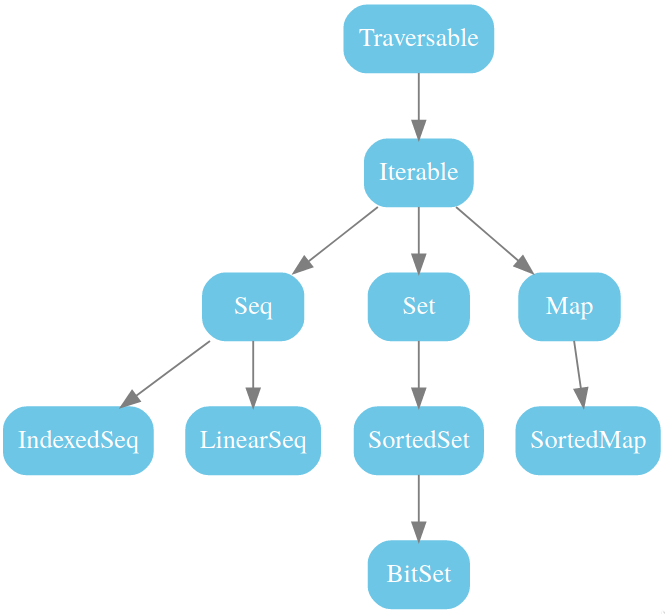
\includegraphics[width=1.0\textwidth]{../img/collection/collection-traits}
\end{Slide}

\noindent Läs mer om Scalas samlingar här: \\ 
\url{http://docs.scala-lang.org/overviews/collections/overview}

\ifkompendium\else

\begin{Slide}{scala.collection.immutable}
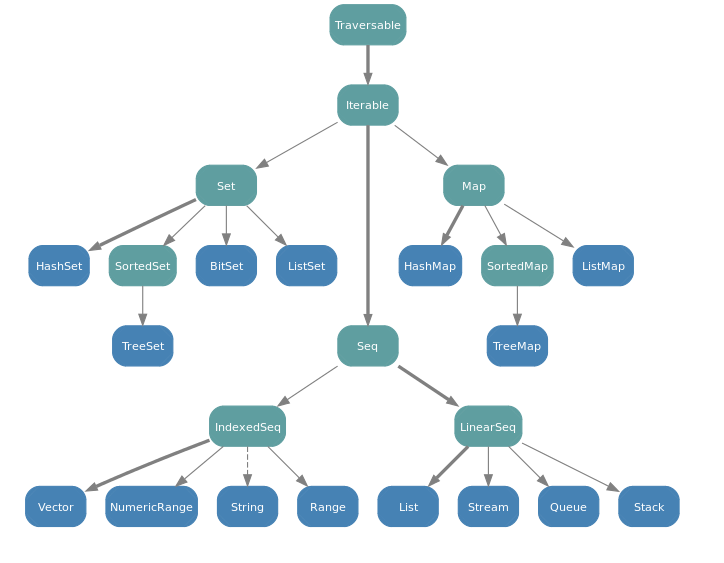
\includegraphics[width=0.82\textwidth]{../img/collection/collection-immutable}
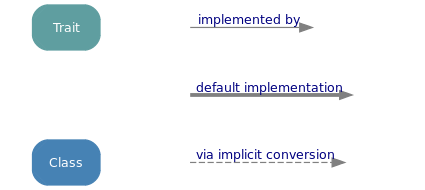
\includegraphics[width=0.33\textwidth]{../img/collection/collection-legend}
\end{Slide}

\begin{Slide}{scala.collection.mutable}
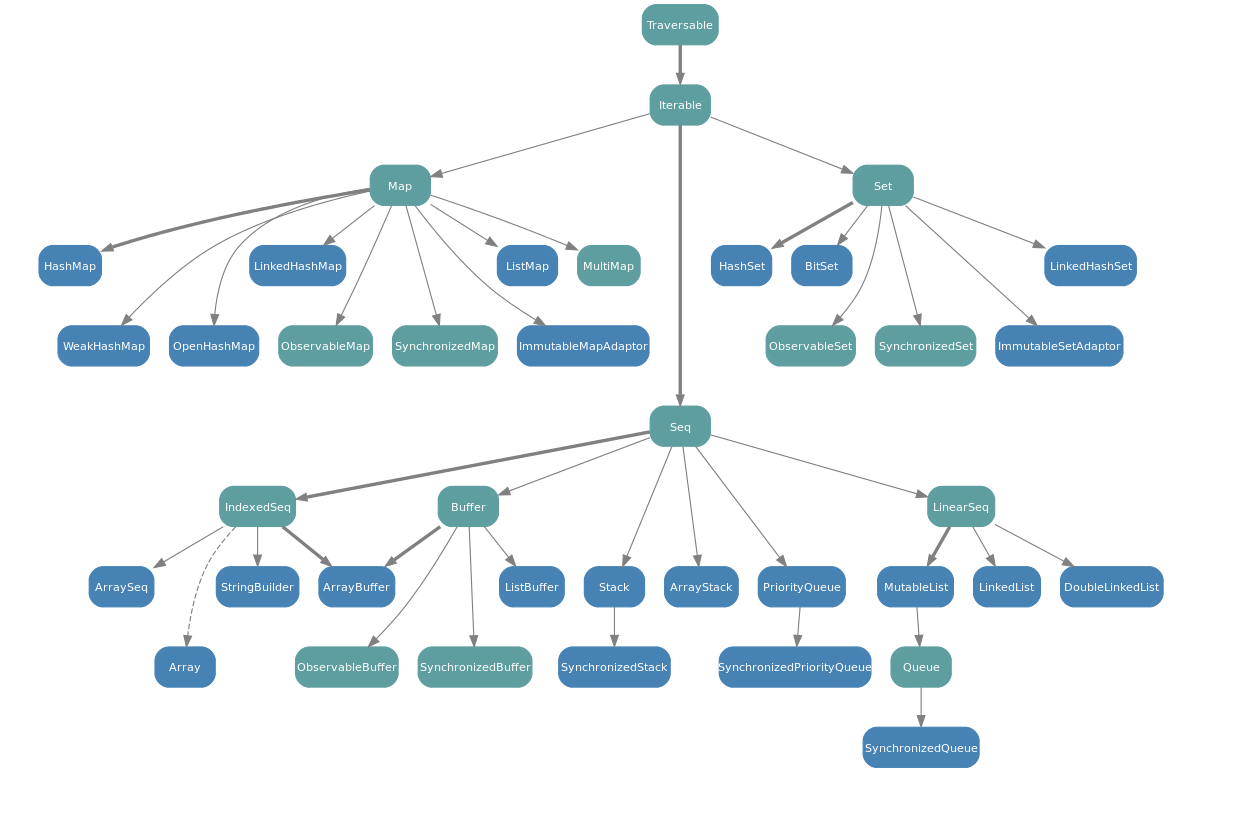
\includegraphics[width=1.05\textwidth]{../img/collection/collection-mutable}
\end{Slide}


\begin{Slide}{Vector eller List???}\SlideFontTiny
\url{http://stackoverflow.com/questions/6928327/when-should-i-choose-vector-in-scala}

''
\begin{itemize}
\item We only need to transform sequences by operations like map, filter, fold etc: basically it does not matter, we should program our algorithm generically and might even benefit from accepting parallel sequences. For sequential operations List is probably a bit faster. But you should benchmark it if you have to optimize.

\item We need a lot of random access and different updates, so we should use vector, list will be prohibitively slow.

\item We operate on lists in a classical functional way, building them by prepending and iterating by recursive decomposition: use list, vector will be slower by a factor 10-100 or more.

\item We have an performance critical algorithm that is basically imperative and does a lot of random access on a list, something like in place quick-sort: use an imperative data structure, e.g. ArrayBuffer, locally and copy your data from and to it.


\end{itemize}
\end{Slide}

\fi






\end{document}
